\documentclass{mcmthesis}
\mcmsetup{CTeX = true,  
        tcn = 1912947, problem = B,                                           
        sheet = true, titleinsheet = true, keywordsinsheet = true,
        titlepage = false, abstract = false}
\usepackage{multirow}
\usepackage{palatino} 
\usepackage{lipsum}
\usepackage{indentfirst}
\usepackage{amsmath}
\usepackage{amssymb}
\usepackage{graphicx, subfig}
\usepackage{caption}
\usepackage{booktabs}
\usepackage[section]{placeins}
\usepackage{geometry}
\usepackage{float}
\usepackage{algorithm}
\usepackage{algorithmic}
\usepackage{setspace}

%\geometry{bottom=2.5cm}
\geometry{left=2cm,right=2cm,top=2.5cm,bottom=2cm}
%\newcommand{\upcite}[1]{\textsuperscript{\textsuperscript{\te{#1}}}}   

%\setlength\parskip{.5\baselineskip}
%\newtheorem{definition}{Definition}[section]

\title{Creative Design Based on Transportable Disaster Response System(DroneGo)}                                        
%\author{\small \href{http://www.latexstudio.net/}
%  {
\includegraphics[width=7cm]{mcmthesis-logo}}}
%\date{\today}
\begin{document}
\begin{abstract}  
	How to transport medical packages and finish reconnaissance task quickly when facing worst disaster and isolated environments is a valuable issue. In this paper, we propose a transportable disaster response system named DroneGo to model this real problem based on the condition of Puerto Rico's hurricane in 2017. \par
	Grids Traversing Model (GTM) is proposed as a basic quantification of the real problem, since the calculation for delivery and detection tasks can be conveniently done within a grids environment. For determining which grid to be detected, we take population density, traffic high way density into calculation for grids weights matrix with the help of Entropy Weighting Model (EWM). The generated matrix and maps benefit the work of flight plan and location. \par
	By using EWM again, we rank the seven types of drones to find out the best drone for delivery and for reconnaissance, which greatly simplify the scope of problems. Then we adopt a heuristic algorithm to solve the 3D container-packing problem and obtain the packing solution with maximum spatial utilization rate.\par
	For the optimum localization problem, we starts from five hospitals and consider all the drone types, screening out B, C, F Drone. Then we analysis three kinds of flight path and obtain the combination of circle map and ellipse map. By constructing two kinds of coverage rates (area and weight) and aiming for increasing them, we figure out three optimum positions for three cargo containers.    \par
	Finally comes the most complex flight plan, which is based on all the previous conclusion. We try our best to simulate three flight plan of containers in A* Algorithm and get some considerable achievements - we find our solution can reconnoitre 83.61\% area of Puerto Rico under the  precondition that three day's delivery task can be guaranteed. 
	
	\begin{keywords}
	Grids Traversing Model; 3D-container-packing Problem; Entropy  \\ \enspace\enspace\indent\enspace\enspace\indent\enspace\enspace\indent\enspace\enspace\enspace   Weighting Model;  Optimum Location Problem; A* Algorithm  
	
	\end{keywords}
\end{abstract}
%\enspace\enspace\indent\enspace\enspace 
    \maketitle                             

    \newpage                              
    \setcounter{page}{1}                    
    \tableofcontents                       
    \newpage                             

    %\section{Introduction}
    \subsection{Background}                         % ��������
    There are 6,000 to 7,000 languages being used all over the world currently, but around half of the world's population are using the most important 15 languages. With the development of globalization, the whole world has changed deeply. The impact of this trend does not only exist in economy and society, but also in language and culture. Nowadays, with the continuous improvement of transportation and communication, most people are able to speak the second language besides the mother language, and the second language plays an important role in traveling abroad and international trade.
    \begin{figure}[!htbp]                                           %��һ��ͼƬ�ij���
        \centering
        \includegraphics[width = .8\textwidth]{introduction.jpg}        %�ģ�ͼƬ�ļ�������
        \caption{The Distribution of Various Language}                                  %�ģ�ͼƬ����������ʾ������
        \label{introduction}                                           %�ģ�ͼƬ�ڳ����е����ƣ����õ�ʱ����
    \end{figure}

    The current geographical distribution of different languages in the world is shown in the figure \ref{introduction}. When considering the total number of language speakers, native speakers, the second language speakers and even the third language speakers should be taken into consideration. The language distribution is complex and diverse, so the statistics on the total number of languages are a complicated job. At present, many experts and scholars have conducted research in this area to explore whether the trend of language distribution tends to be simplification.
    \subsection{Restatement of the Problem}                  % ǰ�˵Ĺ���
    For the increase of the total number of language speakers, we divided them into native speakers and second language speakers for model building. For the geographical distribution of language speakers, we should not only consider the population increase in each country after 5 years, but also the number of speakers who moving to other countries. Analyzing of the various factors of the problem, we consider the problem how to select the site of the International Office in each country as a risk-based site selection analysis:
This problem can be divided into four parts:
    \begin{itemize}         %û�к����ֵ�
      \item Establish an increase model of the total number of language speakers changed with time to predict the change in the total number of language speakers in the next 50 years.
      \item Establish linguistic geography distribution model changed with time and predict the change of the geographical distribution of the language speakers in the next 50 years.
      \item According to the geographical distribution of language speakers, select the international offices to maximize the profits of the office.
      \item Consider changes in the global communication methods and determine whether the number of international offices can be reduced.
    \end{itemize}


    \subsection{Our Work}                           % ������Ҫ���Ĺ���
    In order to make the prediction more accurate, our work is divided into the following four aspects:
        \begin{figure}[!htbp]                                           %��һ��ͼƬ�ij���
        \centering
        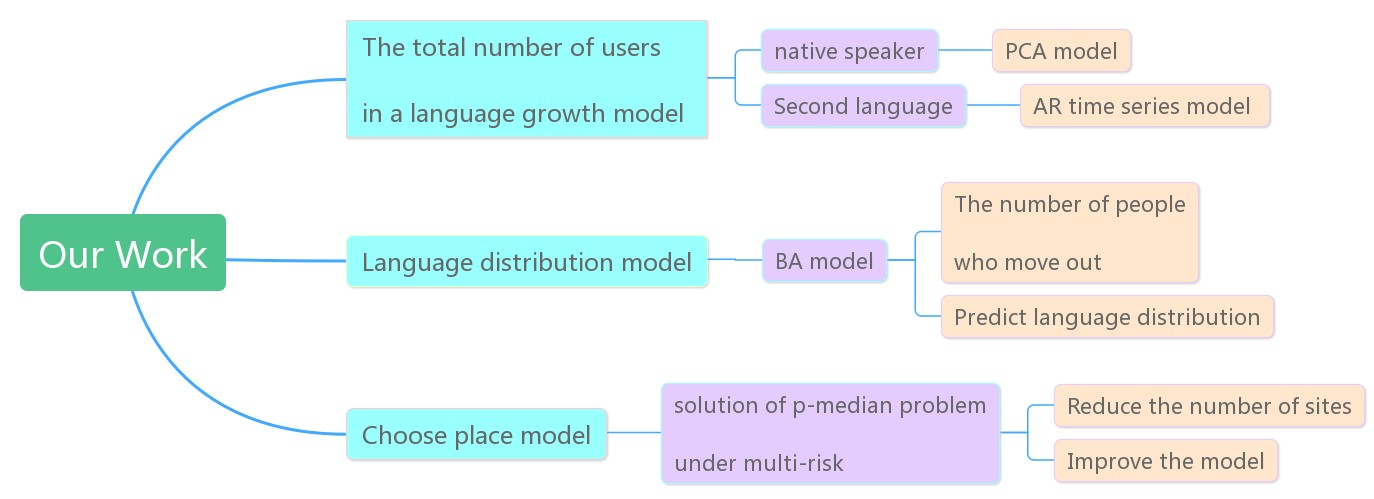
\includegraphics[width = .8\textwidth]{ourwork.jpg}        %�ģ�ͼƬ�ļ�������
        \caption{Flow Chart}                            %�ģ�ͼƬ����������ʾ������
        \label{ourwork}                                           %�ģ�ͼƬ�ڳ����е����ƣ����õ�ʱ����
    \end{figure}


\section{Terminology Explained in Model}        % �൱����������
    \begin{itemize}         %û�к����ֵ�
      \item Nodes centrality degree: The number of edges connected to that node.
      \item L1 country: Countries referred to the country which has Russian as native language.
      \item L2 country: Countries referred to the country which has Russian as second language.
      \item L1 numbers: The numbers of native speakers of a certain language.
      \item L2 numbers: The numbers of second language speakers of a certain language.
    \end{itemize}


\section{Assumptions}
1. We assume that each country uses only the third and fourth languages with very few people, which has little effect on native speakers and second language speakers;

2. We do not consider small probability events in our model, assuming no random events such as world war and economic crisis.

3. Assuming that each country moves in and out of balance, that is, the total population does not change;

4. Assuming that the total number of immigrants to a country speaks the official language of the country and does not consider the issue of the offspring after the move;

5. Assume that all immigrants are legal immigrants;

6. Assuming that national policy does not change significantly over time;

7. Assumptions data are all true and reliable;

\section{Symbols and Definitions}
    \begin{table}[]
    \centering
    \caption{Symbols and Definitions}
    \begin{tabular}{llllll}
             \toprule
        \multicolumn{1}{c}{Symbols} & Meanings                                                                  \\
        \midrule
        ${Y_t}$                     & A country's L1 number                                                         \\
        $\Delta Y(t)$               & the number of population growth one year                                       \\
        $W(t)$                      & A country's L2 speakers                                                       \\
        $S(t)$                      & The population of the country                                                  \\
        ${O_i}$                     & The total degrees of country $i$                                               \\
        ${F_i}(t)$                  & \begin{tabular}[c]{@{}l@{}}The  thrust of\\   country $i$\end{tabular}       \\
        ${N_j}(t)$                  & The attractive force of country $i$                                            \\
        $N{`_i}(t)$                 & \begin{tabular}[c]{@{}l@{}}The tensile force\\   of country $i$\end{tabular}  \\
        ${Q_i}(t)$                  & The total number of people removed from country $i$                            \\
        $R$                         & The total expected value of a local profit                          \\
              \bottomrule
        \end{tabular}
    \end{table}

\section{Simulation Model}                                    % ģ�ͷ�������
    \subsection{Justification of Our Approach}



        \subsubsection{Justification of our approach}
            \begin{itemize}     %��������
                \item \textbf{Why do we build the population growth model?}\\         %ע����ڻ��з��ż���ȥ����
        If we want to model the distribution of language speakers in the future, building the population growth model is necessary because the numbers of different language speakers is changing over time. If we don`t consider this, we can not do the next step and the result must be unreliable.
                \item \textbf{Why do we divide each language into different country?}\\  % ע����ڻ��з��ż���ȥ����
        Because different country has different population growth rule and different L2 country has different proportion of L2 speaker. If we easily add up the native language and the second language and make a simple calculation of population growth model, the error of result is very big.
                \item \textbf{Why do we divide each language into two parts(L1 country, L2 country)?}\\
        It is obviously that L1 country and L2 country have different rule about calculating the proportion of the speakers of a particular language. So what we need do is to find the population of every country which speaks a particular language, and find the proportion of this language in these countries.
            \end{itemize}




    \subsubsection{Basic Model}
    1) AR Time Series Model

In order to get a model which have the ability to predict, we build an AR Time Series Model. Autoregressive model is:
\[\Delta {{\rm{Y}}_{\rm{t}}}{\rm{ = }}{\alpha _{\rm{0}}}{\rm{ + }}\sum\limits_{{\rm{i = 1}}}^n {{\alpha _i}\Delta {Y_{i - 1}} + {\mu _i}} \]


where ${{\alpha }_{0}}$. is constant, ${{\alpha }_{i}}$ is coefficient of the model, ${{\mu }_{i}}$ is White Noise Sequence.

As an analogy, the model of population growth is:

\begin{equation}\label{renkouzengzhang}
  {Y_t} = {Y_{t - 1}} + \Delta {Y_t}
\end{equation}
where ${{Y}_{t}}$ is the population this year, $\Delta {{Y}_{t-1}}$ is the number of population growth, $\left\{ \Delta {{Y}_{t}} \right\}$is first-order difference sequence of the population.

Based on this, the numbers of speakers of a particular language in L1 country are:
\[Y = (1 - \beta  - \lambda ){Y_t}\]
Where $\beta $ is the proportion of immigrant this year,$\lambda $ is the proportion of people with a low level of literacy. $n$is the number of L1 country.

2) PCA Model



    \[\left\{ \begin{array}{l}
{F_1} = {a_{11}}{X_1} + {a_{12}}{X_2} + {a_{13}}{X_3} + {a_{14}}{X_4}\\
{F_2} = {a_{21}}{X_1} + {a_{22}}{X_2} + {a_{23}}{X_3} + {a_{24}}{X_4}\\
{F_3} = {a_{31}}{X_1} + {a_{32}}{X_2} + {a_{33}}{X_3} + {a_{34}}{X_4}\\
{F_4} = {a_{41}}{X_1} + {a_{42}}{X_2} + {a_{43}}{X_3} + {a_{44}}{X_4}\\
{F_5} = {a_{51}}{X_1} + {a_{52}}{X_2} + {a_{53}}{X_3} + {a_{54}}{X_4}
\end{array} \right.\]




    3) Total Numbers of Speakers
    Total numbers of language speakers of a certain language is:
    \[S(t) = Y(t) + W(t)\]
        \subsubsection{ Solution and Result }
        In this problem we have to model the distribution of various language speakers over time. But due to the wide distribution of languages, we focus on the analysis of the four representative languages which are English, Russian, Chinese, Japanese. We use our model to predict their distribution ten years later.


Figure.\ref{sub1} shows the autocorrelation and partial autocorrelation coefficients of Russia`s population growth function, and Figure.\ref{sub2} shows the population trend ten years after the prediction of Russia.

    \begin{figure}[!htbp]                                       
        \centering
        \subfloat[ACF and PACF]{                               
            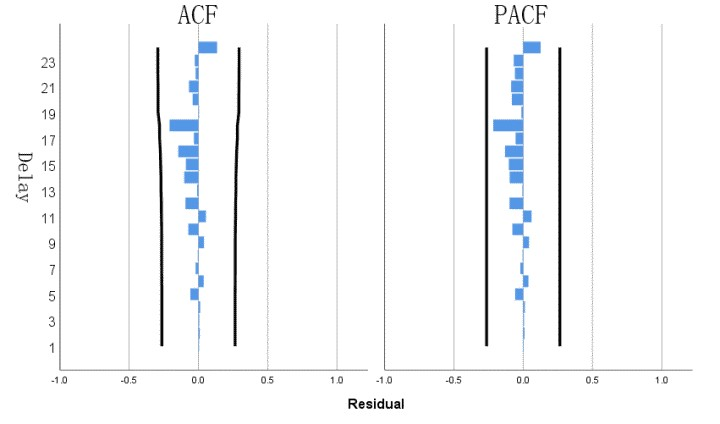
\includegraphics[width = .45\textwidth]{ACF.jpg}
            \label{sub1}                                          
        }
        \qquad
        \subfloat[Change in Russia`s Population]{                            
            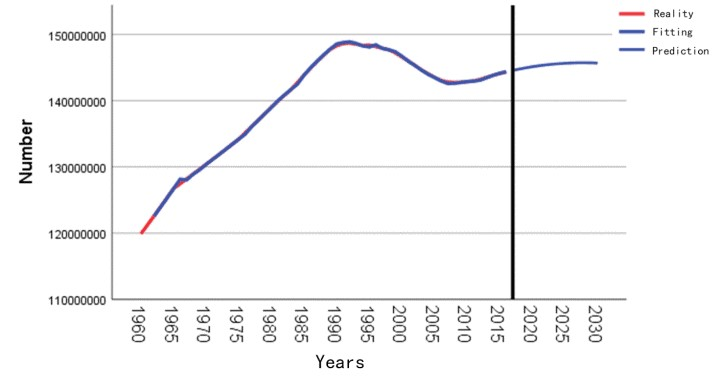
\includegraphics[width = .45\textwidth]{eluosi.jpg}
            \label{sub2}                                            
        }\\ 

        \caption{The Growth Model of Russia`s population}                                       
        \label{eluosibijiaotu}                                 
    \end{figure}

As can be seen from Figure.\ref{eluosibijiaotu}, Russia's total population is 145 million after 10 years. As for $\beta $, $\lambda $ parameter in Equation.\ref{renkouzengzhang}, we find the data from 1960 to 2016 in World bank.

We choose four languages and make a prediction about their L1 speakers number. Result is shown in Table.\ref{Atu}
\begin{table}[H]
\centering
\caption{The Change of L1 Speakers in Four Countries}
\label{Atu}
\begin{tabular}{llllll}
\cline{1-3}
\multicolumn{1}{c}{}        & \multicolumn{1}{c}{Now} & \multicolumn{1}{c}{In ten years} &  &  &  \\ \cline{1-3}
\multicolumn{1}{c}{Russian} & \multicolumn{1}{c}{153} & \multicolumn{1}{c}{162}             &  &  &  \\
\multicolumn{1}{c}{English} & \multicolumn{1}{c}{371} & \multicolumn{1}{c}{405}             &  &  &  \\
\multicolumn{1}{c}{Chinese} & \multicolumn{1}{c}{897} & \multicolumn{1}{c}{955}             &  &  &  \\
\multicolumn{1}{c}{Jpanese} & \multicolumn{1}{c}{128} & \multicolumn{1}{c}{124}             &  &  &  \\ \cline{1-3}

\end{tabular}
\end{table}

As for the number of L2 speakers, we almost find all the certain language`s L2 country and use our model to calculate the number of their L2 speakers in 2017, as is shown in Figure.\ref{AtuL2}. Comparing the result with the actual data in 2017, we find it that our model can basically figure out the number of L2 speakers.
    \begin{figure}[H]                                           %��һ��ͼƬ�ij���
        \centering
        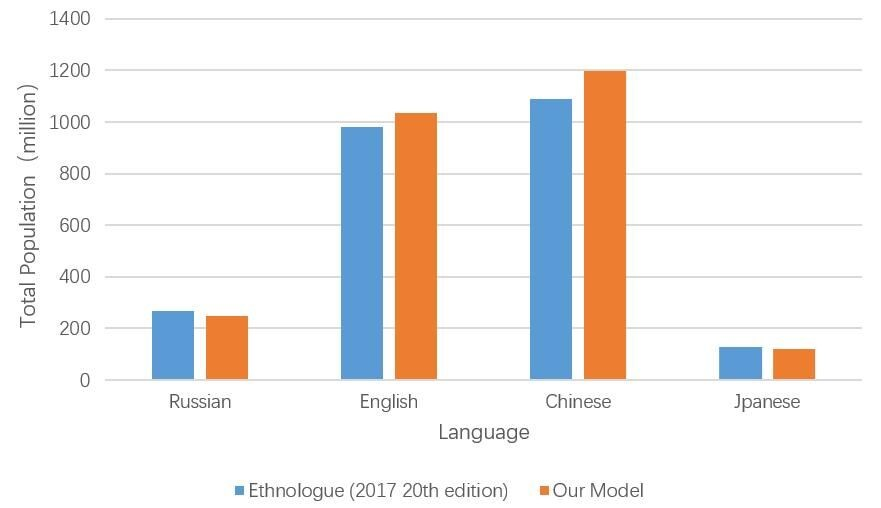
\includegraphics[width = .8\textwidth]{AtuL2.jpg}        %�ģ�ͼƬ�ļ�������
        \caption{Model Test}                            %�ģ�ͼƬ����������ʾ������
        \label{AtuL2}                                           %�ģ�ͼƬ�ڳ����е����ƣ����õ�ʱ����
    \end{figure}

Finally, we predict the total languages speakers of the four languages we choose.

\begin{table}[H]
\centering
\caption{The Total Numbers of Four Languages}
\label{Bjieguo}
\begin{tabular}{cccclcl}
            \toprule
                     & Native Language      &                      & \multicolumn{2}{c}{Second Language}                     & \multicolumn{2}{c}{Total}                               \\
                     \midrule
                     & Now                  & In Ten Years         & Now                  & \multicolumn{1}{c}{In Ten Years} & Now                  & \multicolumn{1}{c}{In Ten Years} \\
Russian              & 153                  & 162                  & 113                  & \multicolumn{1}{c}{119}          & 266                  & \multicolumn{1}{c}{281}          \\
English              & 371                  & 405                  & 611                  & \multicolumn{1}{c}{666}          & 982                  & \multicolumn{1}{c}{1071}         \\
Chinese              & 897                  & 955                  & 193                  & \multicolumn{1}{c}{205}          & 1090                 & \multicolumn{1}{c}{1160}         \\
Jpanese              & 128                  & 124                  & 1                    & \multicolumn{1}{c}{1.2}          & 129                  & \multicolumn{1}{c}{125.2} \\
\bottomrule
\end{tabular}
\end{table}

It can be seen from Table.\ref{Bjieguo} that the total languages speaker change a little after 10 years.

        \subsubsection{Result and Analysis}


\begin{table}[H]
\centering
\caption{The Predictions of 6th-16th Language`s Total Numbers of Speakers}
\label{Bdaan}
\begin{tabular}{ccccccc}
        \toprule
           & \multicolumn{2}{c}{L1} & \multicolumn{2}{c}{L2} & \multicolumn{2}{c}{Total} \\
           \midrule
           & Now    & In 50 Years   & Now    & In 50 Years   & Now     & In 50 Years     \\
Malay      & 77     & 107           & 204    & 271           & 281     & 378             \\
Bengali    & 242    & 340           & 19     & 22            & 261     & 362             \\
Russian    & 153    & 183           & 113    & 158           & 267     & 341             \\
Portuguese & 218    & 297           & 11     & 16            & 229     & 313             \\
French     & 76     & 101           & 153    & 203           & 229     & 304             \\
Hausa      & 85     & 132           & 65     & 93            & 150     & 225             \\
Punjabi    & 148    & 192           &        &               & 148     & 192             \\
German     & 76     & 106           & 52     & 69            & 129     & 175             \\
Persian    & 60     & 84            & 61     & 85            & 121     & 169             \\
Japanese   & 128    & 164           & 1      & 1.3           & 129     & 165.3           \\
Swahili    & 16     & 22            & 91     & 131           & 107     & 153\\
\bottomrule
\end{tabular}
\end{table}


  1. The country corresponding to the top-ten language can be divided into two parts. Some countries have a small population but have developed economically. Some countries have an underdeveloped  economy but have a lager population base.
      \begin{itemize}
        \item As for the first kind of countries like America, they have strong comprehensive national strength so their native language has become world official language, the other country should learn their language to carry out business and other activities.
        \item As for the second kind of countries like China, their people have superiority, so the number of native language is hard to be exceeded by other countries.
      \end{itemize}

  2. Since the countries ranked after the tenth in the rankings are not economy powerhouse and have not a large population base, growth in both native speakers and second language speakers is not high.

      3. We have ignored the small probability events, such as national split, war, invasion by other countries and other factors, so population model is the ideal model, so there will be such a result.



\section{Model II}

    \subsection{Prediction Model}
    1) BA Model



    \begin{figure}[H]                                           %��һ��ͼƬ�ij���
        \centering
        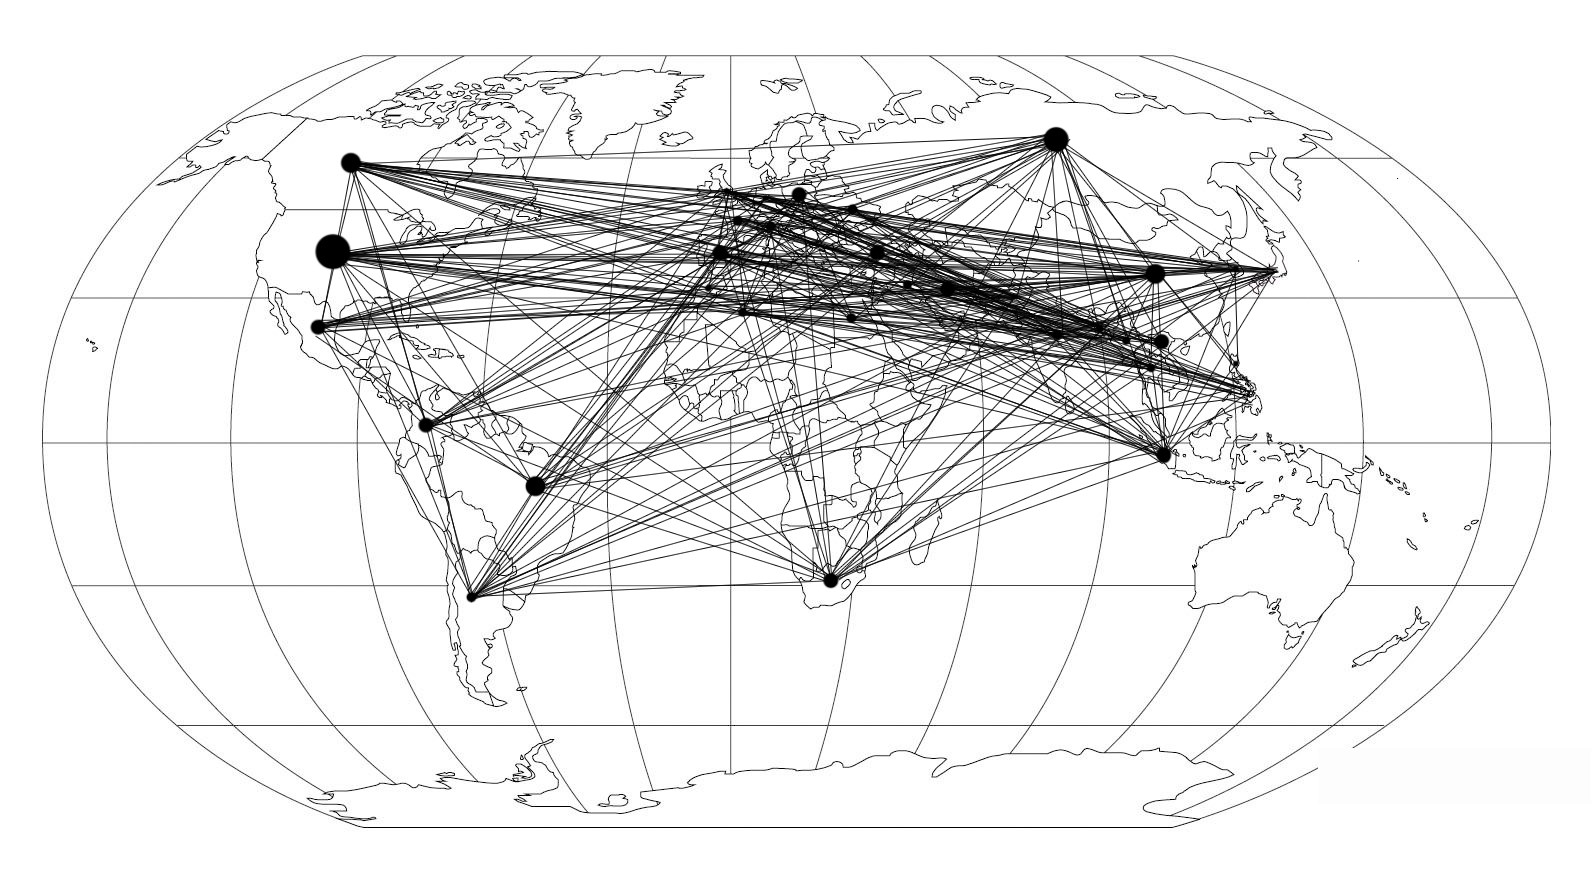
\includegraphics[width = .8\textwidth]{yiduixian.jpg}        %�ģ�ͼƬ�ļ�������
        \caption{Global Population Mobility Network Space Pattern}                            %�ģ�ͼƬ����������ʾ������
        \label{yiduixian}                                           %�ģ�ͼƬ�ڳ����е����ƣ����õ�ʱ����
    \end{figure}





    \subsection{Applications of Our Models}

\section{Strengths and Weaknesses}
    \subsection{Strengths}
        \begin{itemize}
            \item
            \item
            \item
        \end{itemize}
    \subsection{Weaknesses}
        \begin{itemize}
            \item
            \item
            \item
        \end{itemize}

\begin{thebibliography}{99}                 % ���Dz����
    \bibitem{1}
    \bibitem{2}
    \bibitem{3}
    \bibitem{4}
\end{thebibliography}

\begin{appendices}
	
	\section{First appendix}

	
	Here are simulation programs we used in our model as follow.\\
	
	\textbf{\textcolor[rgb]{0.98,0.00,0.00}{Input matlab source:}}
	\lstinputlisting[language=Matlab]{./code/mcmthesis-matlab1.m}
	
	\textbf{\textcolor[rgb]{0.98,0.00,0.00}{Input python source:}}
	\lstinputlisting[language=Python]{./code/feature.py}
	
	\section{Second appendix}
	
	some more text \textcolor[rgb]{0.98,0.00,0.00}{\textbf{Input C++ source:}}
	\lstinputlisting[language=C++]{./code/mcmthesis-sudoku.cpp}
	
\end{appendices}
\end{document}

                      
    \section{Introduction}
    \subsection{Background}                       
	In 2017, the worst hurricane to ever hit the United States territory of Puerto Rico, left the island   severe damage and caused over 2900 fatalities. The combined destructive power of the hurricane's storm surge and wave action produced severe damage to homes, buildings, utility poles, transmission lines, cellular networks, highways and roads. Demands for medical supplies and lifesaving equipment zoomed up while the full extent of the damage remained unclear and dozens of areas were isolated.\par
	Under this background, a non-governmental organizations - HELP, Inc. - is attempting to
	improve its response capabilities by designing a transportable disaster response system called "DroneGo", which is a prologue to this paper. 
	

    \subsection{Clarification of the Problem}             
  We use the 2017 situation in Puerto Rico to design the DroneGo. Four problems wait us to be solved:
    \begin{enumerate}       
    	\item \textbf{Packing configuration of cargo containers:\label{P1}} Recommend a drone fleet and set of medical packages and design the associated packing configuration for each of up to three ISO cargo containers. We have to create a optimization model for the selection scheme since the options are various.
    	\item \textbf{Location of cargo containers:\label{P2}} Identify the best location or locations on Puerto Rico to position one, two, or three cargo containers of the DroneGo. We have to analysis the pros and cons of different quantity of containers and different positions and finally determine the best plan.
    	\item \textbf{Delivery plan:\label{P3}} Design the associated payload packing configurations of the drone fleet, then produce the delivery routes and schedule to meet the identified medical package requirements of the hurricane scenario. We have to choose a comprehensive scheme for both consideration of resources and efficiency.
    	\item \textbf{Reconnaissance plan:\label{P4}} Provide a drone flight plan, enable the DroneGo fleet to use cameras to assess the major highways and roads. We have to create a scientific model to cover as much area of Puerto Rico as possible.
    \end{enumerate}
    
%    
%    \subsection{Our Work}                      
%    In order to make the prediction more accurate, our work is divided into the following four aspects:

    
     \section{Preparation of the Models}
    \subsection{Assumptions}
    1. Neglect small islands around Puerto Rico; \label{as1}
    
    2. Cargo containers are kept in safe places and will not be damaged by disasters. \label{as2}
    
    3. The angle between the visual field of drone's camera and the vertical direction is 60 degrees, the flight altitude of drone is 800 meters and the lines of sight are always straight.  \label{as3}
    
    4. Consider \textbf{three day}'s medical supply delivery tasks and the reconnaissance task only needs to be done once.\label{as4}
    
    5. Because of the loss of power, we \textbf{do not consider the charging of drones}, which means the drones are disposable and we need to prepare three drone fleets for the delivery task.  \label{as5}
    
    6. Assume that if a drone is near a hospital, the drone can land in the hospital and needn't go back. Otherwise, drones must have the capability to come back to the container. \label{as6}
    
    7. The drone's maximum journey distance changes to half when it's full loaded and the affect of payloads on max speed and max flight time are uniform. \label{as7}
    
    8. H Drone is used for communication between the drone fleet and HELP, Inc.'s command and control center.
    \subsection{Variable Declaration} 
    \begin{center}
    	\begin{tabular}{c|l}
    	\toprule[2pt]
    \label{s}
    		\makebox[0.15\textwidth][c]{\textbf{Symbol}}	& \makebox[0.1\textwidth][c]{\textbf{\qquad\qquad\qquad\qquad\qquad\qquad\qquad Definition }}    \\ 	\midrule[1pt]
    		v & Speed of a drone \\ 
    		$t_{max}$ & Maximum flight time no cargo of a drone \\  
    		s  & The maximum journey distance of a drone  \\
    		s1 & The distance from a cargo container to the grid designated \\ 
    		s2 & The distance of traveling a whole small grid \\ 
    		s3 & The distance from the grid to the   nearby hospital \\ 
    		Cr & The coverage rate of grids on Puerto Rico \\ 
    		H  & The flight altitude of drones  \\  
    		R  & The width of visual field of drones' cameras \\
    		S  & The area of each grid \\
    		tt & The maximum time available for a drone to traverse\\
    		&  in the target grid \\
    		Crg & The traversal coverage rate of a drone in a grid \\
    	    $\theta$ & The angle between the visual field of drone's camera and \\
    	    & the vertical direction \\
    		$G(m,n)$ & All grids consist of m rows and n columns \\
    		$N$ & Number of grids (equals to $m*n$) \\
    		$C$  & The number of grids that are covered in our solution\\
    		$THD$ &   The matrix of traffic highway density, which also has \\
    		& m rows and n columns     \\
    		$PD$  &   The matrix of population density, which also has\\
    		&  m rows and n columns \\
    		$mpc$ &   Max payload capability of a drone \\
	$p$   &   The actual payload of a drone \\
$V$   &   The volume of a drone \\
$V'$  &   An index for rating capacity of drones that is related to $V$ \\
$l,w,h$   &   Length, width and height of drones   \\
$bt$  &  The drone cargo bay type \\
    	    $bt'$ &  An index for rating capacity of drones that is related to $bt$  \\
    	\bottomrule[2.5pt]
    	\end{tabular}
    \end{center}

\begin{center}
	\begin{tabular}{c|l}
		\toprule[2pt]
		\makebox[0.15\textwidth][c]{\textbf{Symbol}}	& \makebox[0.1\textwidth][c]{\textbf{\qquad\qquad\qquad\qquad\qquad\qquad\qquad Definition }}    \\ 	\midrule[1pt]
    $\alpha$ & Coverage rate of grids number  \\
    $\beta$ & Coverage rate of grids weights \\
    	\bottomrule[2.5pt]
\end{tabular}
\end{center}
    \section{Grids Traversing Model (GTM)}                                    
    The DroneGo is made up of two parts - delivery system and reconnaissance system - both of which can be finished by drones. By doing some estimate, we find the daily delivery task can be easily satisfied while the reconnaissance task are hard to achieve. So we propose Grids Traversing Model firstly, which are aimed at \textbf{reconnoitring} as much area as possible and determining the optimum \textbf{location}.
\subsection{Grids Partition}
 Obviously, the maximum stroke of a drone is very limited (less than 52.66km). To reconnoitre more area, we can set the scanning task of each drone in one appropriate grid. Each drone mainly needs to reconnoitre several grids (of course plus the route it travels) and comes back so that it's convenient to make the flight plan.
    \subsection{Determine the Grid Size}  
    \subsubsection{Grid Constraints} 
    The grid is supposed to meet the following constraints:
    	\begin{enumerate}
    		\item The size must be appropriate for the drone to finish traversing task in limited time.  
    		\item Grids must be regular graphics, better be rectangle or even square, which are easily to be partitioned and traversed. 
    		\item All grids have the same size and no overlap exists.
    		\item Grids must cover every area as much as possible, and the coverage rate $Cr$ must be greater than 90\%. 
    		
    	\end{enumerate} 
    \par
   	 Besides, to determine the size of a grid, we have to calculate the width of drone's field of vision. We propose the next model to quantify it.
  
   	\subsubsection{Simple Cone Model }
   	Assume cameras of drones face down, then the surface surrounded by visual field and the ground make up a cone. Figure \ref{1} shows the detail\cite{1}.
   	 \begin{figure}[H]                                         
   		\centering
   		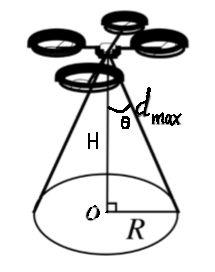
\includegraphics[width = .2\textwidth]{capture.PNG}      
   		\caption{ A Drone's Fight View }                            
   		\label{1}   
   	\end{figure} 
   	The diameter of bottom circle determines how big area the drone can reconnoitre in limited time. If a drone has time $tt$ to traverse in the grid, then its maximum traversal area is $2*R*v*tt$. The $R$ is equal to $H*tan\theta $. Then we have the following formula for calculating the traversal coverage rate in a grid:
   	\begin{equation} 
   			Crg=2R*v*tt/S 
   	\end{equation}
   	To get bigger $Crg$, smaller $S$ is better, but smaller $S$ means there are more grids, which may increase the complexity of fight plan. 
   	In addition, We don't take it into consideration that the turning distance may cause loss and the drone may need to come back to the place entering the grid from the place traversing all the grid. Besides, the traversing route is S-shaped.\par
   	According assumption 3, the flight altitude is 800 m and $\theta$ is 60 degrees, which determine the width of field of view is $2*800* tan 60^\circ \approx 2770 m.$ 
   	After some comprehensive calculation and bold estimate, we determine to construct $12*35=420$ square grids whose edge length is 5 km. Figure \ref{gp} shows the specific segmentation.
   	    \begin{figure}[H]                                         
   		\centering
   		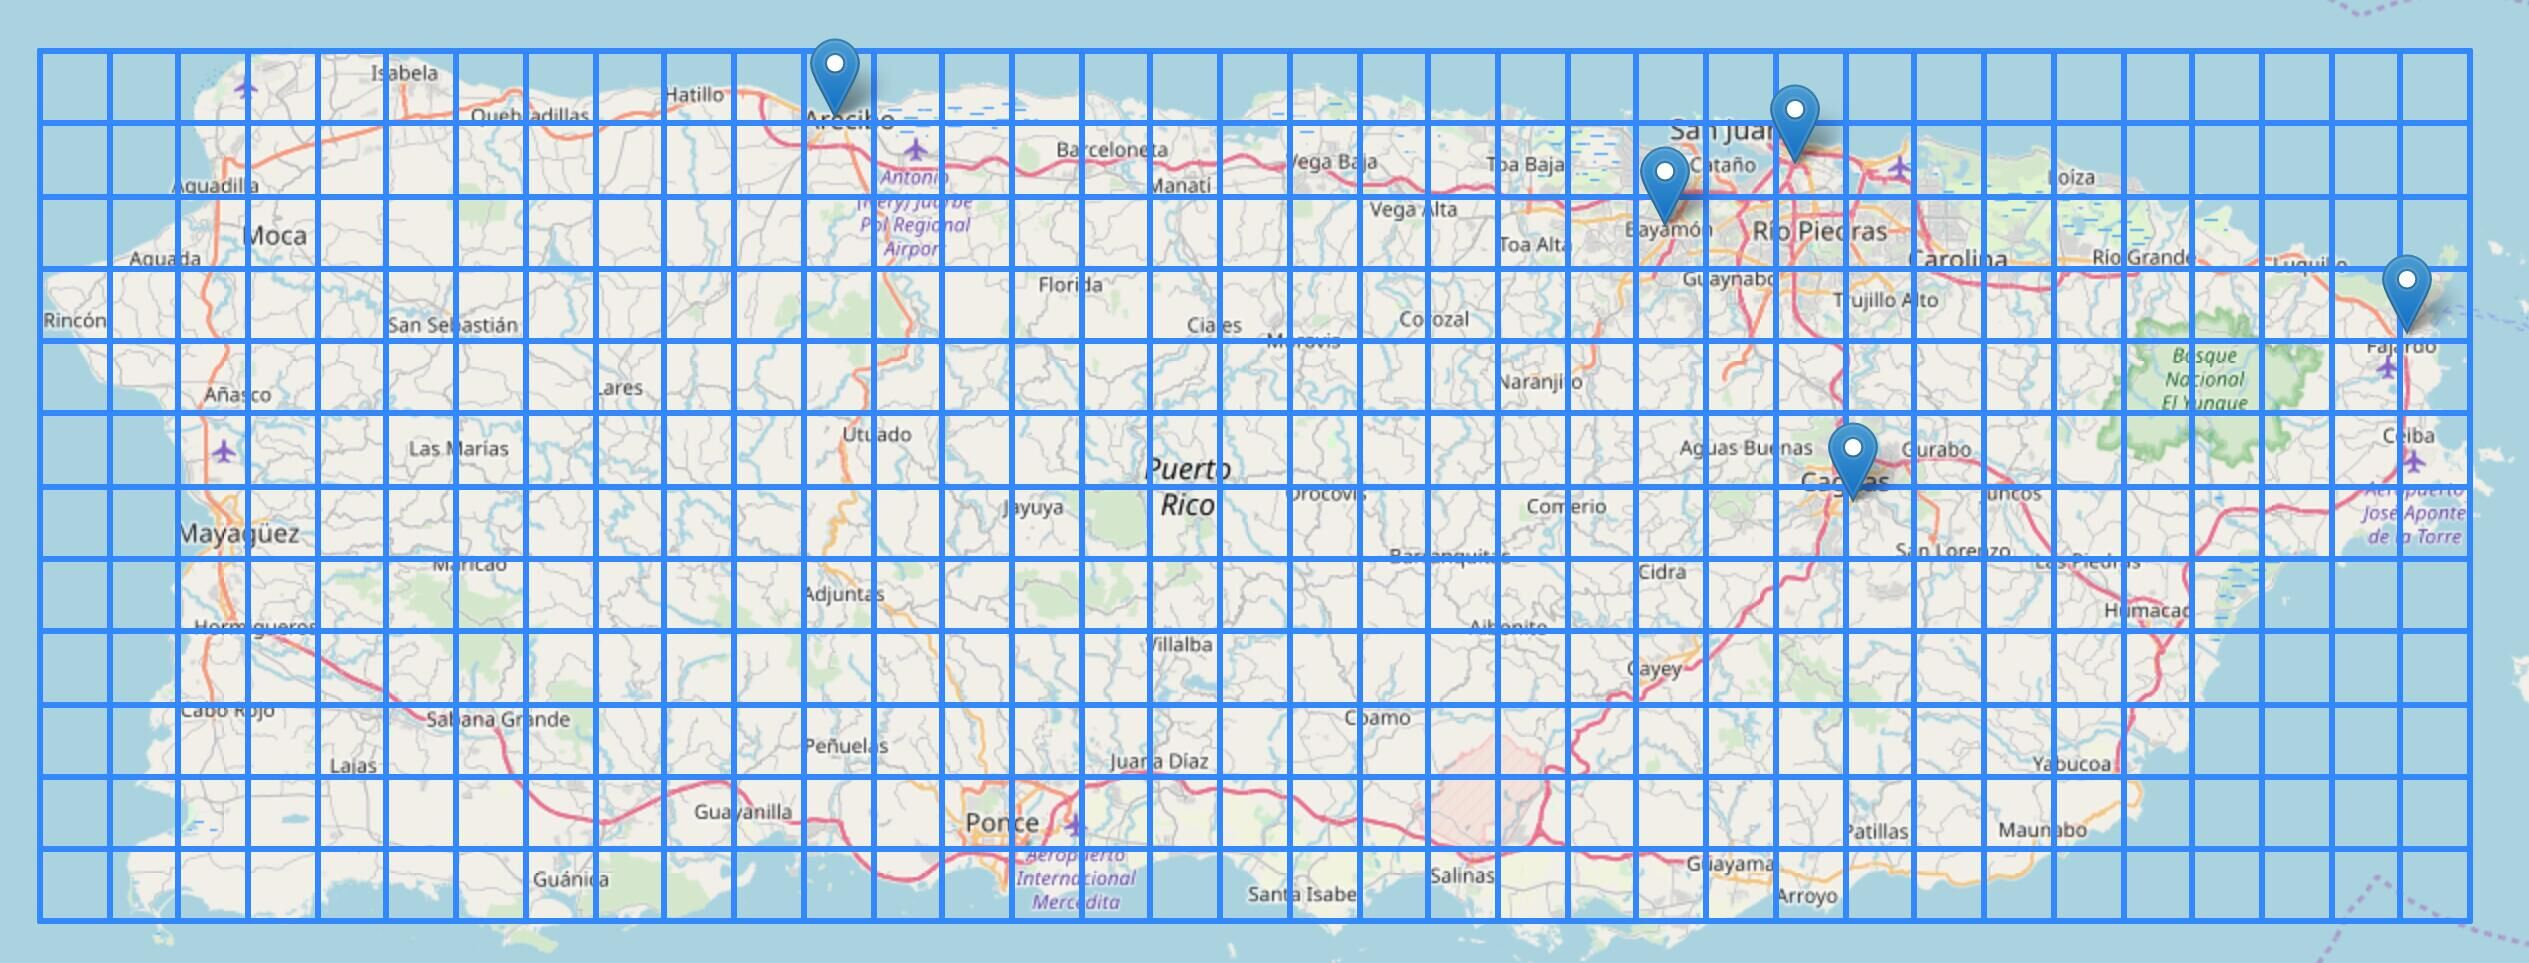
\includegraphics[width = .8\textwidth]{grids.jpg}      
   		\caption{Grids Partition (12 rows * 35 columns) }                            
   		\label{gp}                                          
   	\end{figure}
   
   \subsection{Grids Weights Assignment}
   The partitioned grids are not only beneficial for providing a drone flight plan(Problem \ref{P4}), but also for the resolution of optimum location(Problem \ref{P2}). Since the number and capacity of drones are not enough to traverse the whole Puerto Rico Area, we can set a weight to each grid. In this way, we can give priority to grids with high weights and locate the cargo contain where most high weighted grids can be reconnoitred.\par
   We consider two factors to influence the weights of grids: traffic highway density and population density. After that we use entropy weighting model(see section \ref{EWM}) to take the two factors into account and generate the final weights form(or matrix).
   \paragraph{Traffic Highway Density }
   The highway density in a grid can indicate how important the grid is deserved to be reconnoitred. We can use formula \ref{hh} to calculate each grids' density\cite{2}:
   \begin{equation}  \label{hh}
   V=\sum\limits_{i=1}^4{Q_i}= \sum\limits_{i=1}^4 {C_i\alpha_i\beta_i\gamma_iN_iL_i}
   \end{equation}
   In this formula, $V$ means the total throughput of road network(pcu
   ${{\cdot}}$km/h), which can represent the traffic highway density. $Q_i$ means the throughput of class i road. i equals to 1 $\sim$ 4 which represent expressway, main road, secondary road and Access Rd. $C_i$ means accessible capacity of single lane on class i road. $\alpha_i$ means the saturation of class i road. $\beta_i$ means reduction coefficient at intersection of class i road. $\gamma_i$ means the lane comprehensive reduction coefficient of class i road. $N_i$ means the average number of motor vehicle lanes of class i road. $L_i$ means the mileage of class i road(km).  
   
   Due to time and data limitation, we grade each grid with a rank (0$\sim$3) according to the above factors as figure \ref{thd} shows. Grade 0 represents it's low density while grade 3 means high density. Figure \ref{tdm} shows the concentration of traffic density.
	   \begin{figure}[!htbp]                               
		\centering
		\subfloat[Traffic Density Grade Evaluation ]{                             
			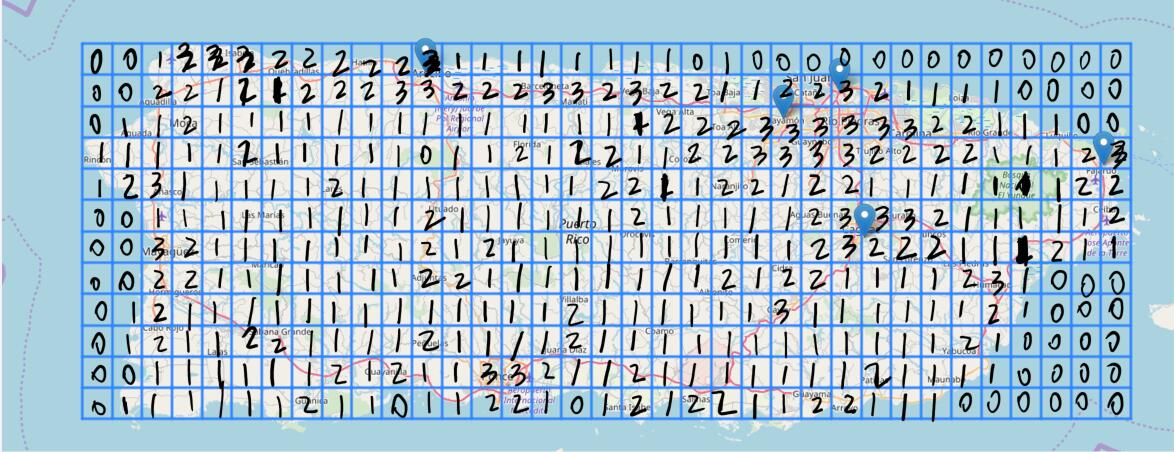
\includegraphics[width = .45\textwidth]{jt2.jpg}
			\label{thd}  		                                        
		}
		\qquad
		\subfloat[Traffic Density Map ]{                               
			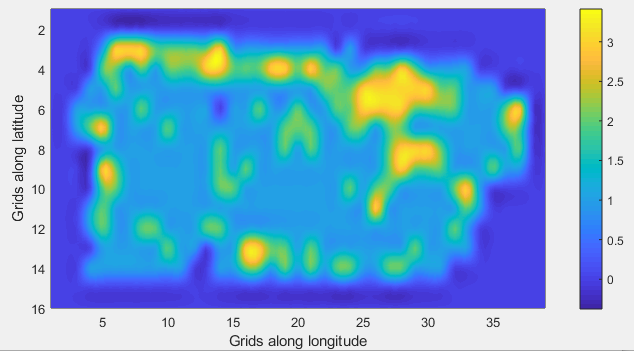
\includegraphics[width = .45\textwidth]{jt.png}  
			\label{tdm}                                          
		}\\ 
	\caption{Traffic Highway Density Grade and Concentration Picture}                             
\end{figure}
    \paragraph{Population Density}
    We can find some population data of Puerto Rico's 78 cities and the total population data over the years in \cite{3} and \cite{4}. By regional population underestimate, we can also obtain the population matrix containing each grids' population value. The figure \ref{cmdp} shows our result. \par
    
       \begin{figure}[!htbp]                                         
    	\centering
    	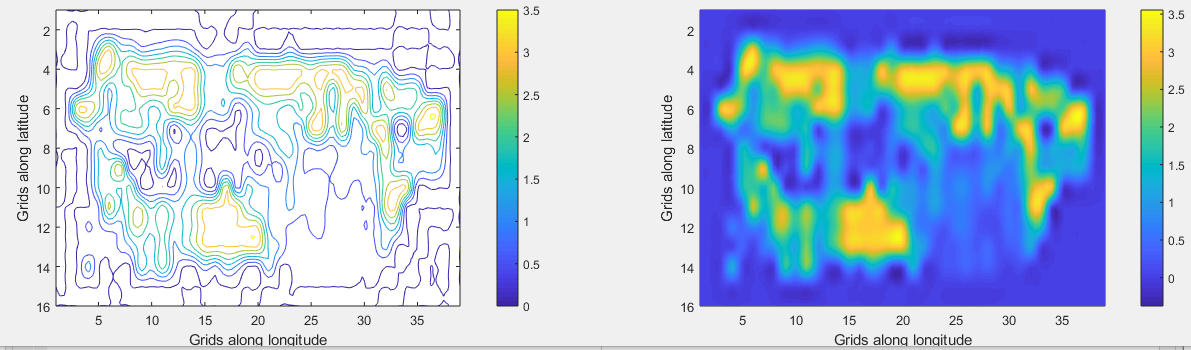
\includegraphics[width = .8\textwidth]{rk.png}      
    	\caption{ Contour map and Density of Population }                            
    	\label{cmdp}                                          
    \end{figure}
    So far, we get two density map which is helpful for the selection of optimum container location. Two matrix $THD$ and $PD$ are built, which can be the input of next model - \textbf{Entropy weighting model(EWM)}(see section \ref{EWM}) - and finally we obtain that the population density to traffic highway density ratio is \textbf{0.6172 to 0.3828} and produce the grids weights matrix. 
     We use \textbf{python} to calculate the whole calculation process and use \textbf{matlab} to carry out visualization. Figure \ref{finalweights} is part of our result. For making the gap more obvious, we multiply each value by 1000 thus the sum of weights is equal to 1000. For some areas which are inaccessible such as high mountains, we set the weights of these grids to zero. By the way, the three concentration maps will benefit for containers location while the grids weights matrix will benefit for making reconnaissance plan. 
    	   \begin{figure}[!htbp]                               
    	\centering
    	\subfloat[A Part of the Grids Weights Matrix ]{                             
    		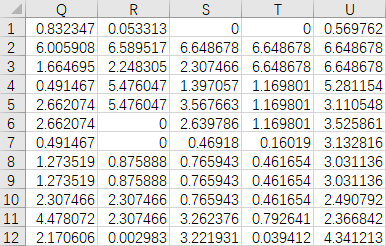
\includegraphics[width = .45\textwidth]{finalweighs.png}
    		\label{finalweights}  		                                        
    	}
    	\qquad
    	\subfloat[Concentration of Grids Weights]{                               
    		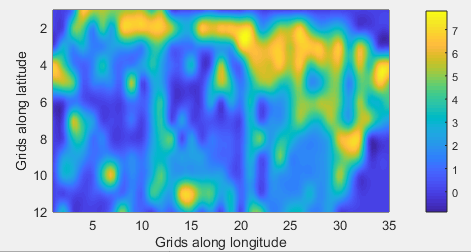
\includegraphics[width = .45\textwidth]{fw.PNG}  
    		\label{thd2}                                          
    	}\\ 
    	\caption{Traffic Highway Density Grade and Concentration Picture}                             
    \end{figure}

    \section{Entropy Weighting Model (EWM)} 
    \label{EWM}
      Entropy Weighting Model is aimed at calculating weights. For a matrix with i rows and j columns(i means the number of samples and j means the evaluation index quantity), we want to give a weight to every evaluation index and rank all the samples. In DroneGo, we have two evaluation index: traffic density and population density, which means j equals to 2. And i can mean the number of grids($m*n$).
    There are mainly three steps in this model: normalization processing, entropy calculation, weights and ranks generation \cite{5}.

   \subsection{Normalization Processing}
   We use the followed formula to do standardization:
   \begin{equation}
   {{\rm{R}}_{i,j}} = \frac{{{R_{i,j}} - {{{\mathop{\rm minR}\nolimits} }_j}}}{{\max {R_j} - \min {R_j}}}
   \end{equation}
   R means the raw matrix, which consists of $THD$ and $PD$. But we need to transfer $THD$ and $PD$ to two column vectors. $R_j$ mean a column vector($THD$ or $PD$). "max" and "min" mean the maximum and minimum value of the column vector. To achieve normalization, the sum of a column vector must be equal to 1. So we only need to divide each value by the sum of the column it belongs to.
     
   \subsection{Entropy Calculation}
   Use $E_j$ expresses the total contribution of all samples to the evaluation $j$, which is calculated by the formula \ref{ej}.
   \begin{equation}
   \label{ej}
   {E_j} =  - K\sum\limits_{i = 1}^N {{R_{i,j}}\ln {R_{i,j}}} 
   \end{equation}
   $N$ means the number of grids($m*n$). $K = \frac{1}{{\ln (N)}}$, which is to ensure that $E_j$ belongs to 0$\sim$1. When the contribution value in $R_j$ tend to be consistent, $E_j$ is close to 1. Otherwise, $E_j$ is close to 0. 
     \subsection{Weights and Ranks Generation}
   Use formula \ref{dw} to calculate the weights. $J$ means the number of evaluation indexes.
   \begin{equation}
   {W_j} = \frac{{1 - {E_j}}}{{\sum\limits_{j = 1}^J {(1 - {E_j})} }} \label{dw}
   \end{equation}
   Finally, we can calculate the score of each sample(each grid) and rank them if necessarily.
   Take traffic highway density and population density as an example, the whole flow of $EWM$ is shown in Figure \ref{liucheng}.
      \begin{figure}[!htbp]                                         
    	\centering
    	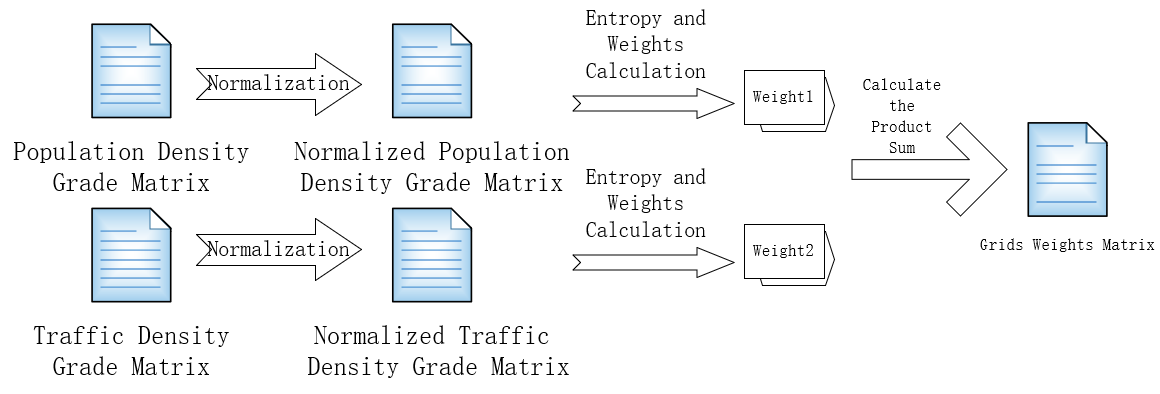
\includegraphics[width = .9\textwidth]{liucheng.PNG}      
    	\caption{ EWM Flow  }                            
    	\label{liucheng}                                          
    \end{figure}
  
  \section{Resource Allocation Model (RAM)}
  For the purpose of recommending a reasonable drone fleet, set of medical packages and packing configuration(Problem \ref{P1}), we can rate each type of drone firstly with the help of \textbf{EWM}, which can obtain the comprehensive capability of drones in medical supply delivery and video reconnaissance. Then we use a set of heuristic algorithms to solve the 3D Bin Packing Problem. Please note that here we choose \textbf{3 cargo containers} to calculate directly and already know the positions of containers. The detailed reason is shown in section \ref{ols}.
  
  \subsection{Drones Rating Method}
  \label{ldis}
  The \textbf{flying range of drones} is our first focus. We think that the range is the most important index when we choose drones. According to assumption 7, we have the following equation to calculate the maximum loaded flying range:
  \begin{align}
  \label{8}
  {v_{loaded}} &= \sqrt {1 - \frac{1}{2}\frac{p}{{mpc}}} v\\
  {t_{loaded}} &= \sqrt {1 - \frac{1}{2}\frac{p}{{mpc}}} {t_{\max }}\\
  s &= {v_{loaded}}*{t_{loaded}}
    \label{dc}
  \end{align}
%  \begin{equation} 
%  s = \sqrt {1 - \frac{1}{2}\frac{p}{{mpc}}} v*\sqrt {1 - \frac{1}{2}\frac{p}{{mpc}}} {t_{\max }}
%  \end{equation}
   In the rating process, we use the average weight $p$ = 6 pounds of the medical kits that each hospital needs every day to calculate $s$ with payloads. Since the max payload capability of A Drone is 3.5 (less than 6), we set its medical supply task capacity rate to 0.
   
   The dimension of drones is an important index. We can use $V=l*w*h$ to describe the size of drones. The longest edge of drones is also a meaningful variable. But there is obvious difference between it and $V$, we ignore it in rating method. In order to make full use of the container space, it's better if the size of drones for reconnaissance is smaller. Hence we use \textbf{the reciprocal of $\mathbf{V}$} as a rating index. Furthermore, the changing range of rates is an important variable affecting the weights in the subsequent information entropy calculation, so we control the changing range of rates in $V$ by \textbf{power reduction operation}, which makes the changing range of rates in $V$ equals to that in $s$. The final formula using data $V$ is:
   \begin{equation}
   V' = {(\frac{1}{V})^{\frac{2}{3}}} = {(\frac{1}{{l + w + h}})^{\frac{2}{3}}}
   \end{equation}
   For the configuration capabilities indexes, if drones do not have the ability to do a task, then the rate of this kind of drones in this task index is 0. Particularly for \textbf{bay type} index $bt$, we increase its changing range by increasing the power in like manner as operation on $V$: $ \mathbf{bt'}=bt*bt$. \par
   With the description above, we generate a normalized drones attribute matrix with four indexes shown in Figure \ref{tdge}. 
      \begin{figure}[!htbp]                               
   	\centering
   	\subfloat[Attributes of Drones on Four Indexes]{                             
   		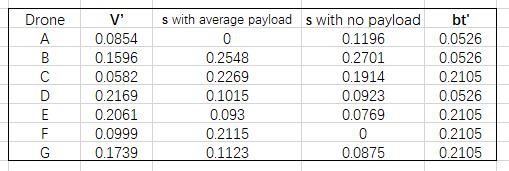
\includegraphics[width = .45\textwidth]{rate.png}
   		\label{tdge}  		                                        
   	}
   	\qquad
   	\subfloat[Final Scores of Drones on Two Tasks ]{                               
   		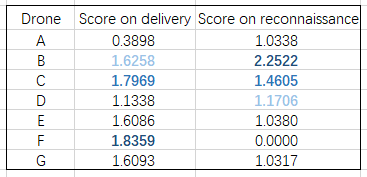
\includegraphics[width = .45\textwidth]{finalRate.png}  
   		\label{fsd}                                          
   	}\\ 
   	\caption{Attribute Matrix and Rating Results} 
\end{figure}
\par
	Now we can calculate the weights of indexes under different tasks with the help of \textbf{EWM}.  
	\textbf{For delivery task}, we consider three dimensions:  $s$ with average payload, $V'$ and $bt'$. Use these three columns of data in Figure \ref{tdge} as the input of EWM to calculate the weights of the three index. The result is: weight\_$s$(0.4130), weight\_$V'$(0.2470), weight\_$bt'$(0.3400).
	\textbf{For reconnaissance task}, we consider two dimensions: $s$ with average payload, $V'$ ($V'$ is necessary since it can affect how many drones the cargo contains can accommodate). Use the two columns from Figure \ref{tdge} as the input of EWM to calculate the weights of the two indexes. The result is: weight\_$s$(0.6879), weight\_$V'$(0.3121). These results verify that our conjecture that maximum journey distance $s$ is the most influential variable. \par
	Then use the following two equations to calculate the final scores of each type of drone on two tasks.
	\begin{align}
	Score_{delivery}&=weight\_s * s_{with\_payload} + weight\_V' * V' + weight\_bt' * bt' \\
	Score_{reconnaissance}&=weight\_s * s_{with\_no\_payload} + weight\_V' * V'
	\end{align}
%	\begin{equation}
%	Score_{reconnaissance}=weight\_s * s_{with\_no\_payload} + weight\_V' * V'
%	\end{equation}
	The final scores of each drone is shown in Figure \ref{fsd}. It's clear to see that \textbf{F Drone} is best suited for delivery task and \textbf{B Drone} is best suited for reconnaissance task.
	
	\subsection {Drones and Containers  Configuration for Packing}
	From the result of drones rating method above, we decide to pack as many B drones as possible with the prerequisite that there are three sets of medical packages and drone fleets that could ensure the resource available for three day's delivery task (Assumption 4). From the analysis of OLM (section \ref{ols}), we obtain the position of three containers. Hence it's easy to determine which container responsible for delivery of corresponding hospitals, and then determine which types of drones, how many drones to do delivery tasks. As for the routes and schedule, we expect all the drones take the air (shortest) line to hospital. Then we can calculate the fight time according to equation \ref{8} to \ref{dc}. The drones' payload packing configuration and schedule are shown in Table \ref{dcp}. 
	\begin{table}[H]
		\centering
		
		\begin{tabular}{lllcc}
			\cline{1-5}
			
			\multicolumn{1}{c}{Hospital (abbr.)}  & \multicolumn{1}{c}{Container}         & \multicolumn{1}{c}{Drone} & \multicolumn{1}{c}{Distance (km)}     & \multicolumn{1}{c}{Fight Time (hour)} \\
			\cline{1-5}
			
			\multicolumn{1}{c}{CMC}  & \multicolumn{1}{c}{3}  &\multicolumn{1}{c}{B: 1*3}    & 36 & 0.55   \\
			\multicolumn{1}{c}{HH}   & \multicolumn{1}{c}{3}  &\multicolumn{1}{c}{E: 1*3}    & 7 &  0.14  \\
			\multicolumn{1}{c}{HPS}  & \multicolumn{1}{c}{3}  &\multicolumn{1}{c}{B: 1*3}  & 27 & 0.39 \\ 
 			\multicolumn{1}{c}{PRCH} & \multicolumn{1}{c}{3}  &\multicolumn{1}{c}{B: 1*3;  C: 1*3}  & 28 & B: 0.448; C: 0.494     \\
 			\multicolumn{1}{c}{HPA}  & \multicolumn{1}{c}{1}  &\multicolumn{1}{c}{B: 1*3}   & 32  & 0.43  \\ 			
			\cline{1-5}
			
		\end{tabular}
		\caption{Drone Payload Packing Configuration and Schedule}
		\label{dcp}
	\end{table}
	The column "Container" means the container charging for the appointed hospital: No.1 means $(18.20^\circ N, 65.97^\circ W)$, No.2 means $(18.20^\circ N, 66.50^\circ W)$, No.3 means $(18.20^\circ N, 65.97^\circ W)$. The "*3" in column "Drone" means three day's quantity. Distance to CMC is not the shortest path since there are a mountain high more than 3000 m. From column "Flight Time" we can see the quickest time for finishing the delivery task is 0.55 hour. \textcolor[rgb]{1.00,0.00,0.00}{Now, Problem \ref{P3} has been solved.}
	   
	Now the numbers and types of basic drones and medical kits for three delivery tasks are clear, we can focus on how to pack the cargo into three containers so that more area can be reconnoitred under limited resource. For achieving the max spatial utilization rate, we regard this problem as a three-dimensional packing problem and refer to the following algorithm \cite{6} to get the answer of containers configuration. Two related algorithms are shown in appendix A. Finally, we obtain the final configuration of ISO cargo containers as shown in Table \ref{pctc}.  \textcolor[rgb]{1.00,0.00,0.00}{Now, Problem \ref{P1} has been solved.}
%	\begin{algorithm}[htb]
%		\setstretch{1.35} %??????????????????1.35??
%		\caption{}
%		\label{alg:Framwork}
%		\begin{algorithmic}
%			\REQUIRE ~~\\
%			The set of positive samples for current batch, $P_n$;\\
%			The set of unlabelled samples for current batch, $U_n$;\\
%			Ensemble of classifiers on former batches, $E_{n-1}$;
%			
	
%			\ENSURE ~~\\
%			
%		\end{algorithmic}
%	\end{algorithm}




\begin{algorithm}
	\label{al1}
	\renewcommand{\algorithmicrequire}{\textbf{Input:}}
	\renewcommand{\algorithmicensure}{\textbf{Output: }}
	\caption{3D Bin Packing Heuristic Algorithm}
	\begin{algorithmic}[1]
		\REQUIRE  Size of containers, drones and medical packages; Number of indispensable containers and medical packages for three day's delivery task.
		\ENSURE Loaded cargo quantity with the types.
		\STATE Denote the set of n items as I. Each item is of length $l_i$, height $h_i$ and width $w_i$. 
		\STATE Initialize a sufficiently large bin(B) with length L, width W, height H (We could set 
		$L = W = H = \sum\limits_{i = 1}^n {\max ({l_i},{h_i},{w_i})} $).
		\STATE Initialize the set of remaining items $I' = I$ and the set of empty maximal spaces as $ES = \phi$.
		\FORALL {$t$ = 1 to $n$}
		\STATE   \textbf{if} t=1 \textbf{then}
		\STATE   Select an item with largest surface area.
		\STATE Put the item into the    bin and generate 3 empty maximal spaces ES1. Update ES = ES1.
		\STATE  \textbf{else}
		\STATE Select a item i from set S according to least waste space heuristic(Algorithm 3). Update 
		$ I' \leftarrow I'\backslash i$.
		\STATE  Select an empty maximal space from ES and decide the orientation according to Least surface Area Heuristic(Algorithm 2). 
 		\STATE  Generate new empty maximal spaces(ES1) and delete those that are intersected and overlapped(ES2). Update $ES \leftarrow ES \cup ES1\backslash ES2$.
 		\STATE \textbf{end if}
		\ENDFOR
		\STATE \textbf{Return} loaded cargo quantity with the types.

	\end{algorithmic}  
\end{algorithm}

\begin{table}[H]
	\centering

	\begin{tabular}{llll}
		\cline{1-4}
		
		\multicolumn{1}{c}{Container}  & \multicolumn{1}{c}{Position} & \multicolumn{1}{c}{Drone Configuration} & \multicolumn{1}{c}{Medical Kits Configuration} \\ 
		\cline{1-4}
		
		\multicolumn{1}{c}{1} & \multicolumn{1}{c}{$(18.29^\circ N, 66.97^\circ W)$} & \multicolumn{1}{c}{B:75 G:1 H:1}    &  $M_1\times3+M_n\times n$     \\
		\multicolumn{1}{c}{2} & \multicolumn{1}{c}{$(18.20^\circ N, 66.50^\circ W)$} & \multicolumn{1}{c}{B:75 G:1 H:1}   &   $M_n \times n$      \\
		\multicolumn{1}{c}{3} & \multicolumn{1}{c}{$(18.20^\circ N, 65.97^\circ W)$}  &\multicolumn{1}{c}{B:61 C:3 E:3 H:1}   &  $M_1\times 18+M_2\times 6 +M_3 \times 12 +M_n\times n$ \\ 
		
		\cline{1-4}
		
	\end{tabular}
	\caption{Packing Configuration for Three Containers}
		\label{pctc}
\end{table}
We find there are space for containing hundreds of medical packages, so we don't give specific data about it. $M_n \times n$ means there are medical packages for more than one week's demands.
	
    
    
    \section{Optimum Localization Model (OLM)} \label{ols}
    
    \subsection{Optimum Container Number}
    The maximum flight distance among all types of drones is about 52.66 km, while Puerto Rico is about 170 km long and 60 km wide. If drones come back to their starting point, they are up to 26 km away from their starting point and then have to come back. What's more, drones' main task is to finish the reconnaissance work of several allocated grids, which needs more traversal time. By drawing a reachable circle area with a corresponding size on the map(the next few pictures show it), it's easy to discover there will be vast areas that cannot be reconnoitred if there are only one or two cargo containers. Therefore, we decide to arrange \textbf{three containers}, which may ensure 70\% of Puerto Rico can be probably reconnoitred by rough estimates. 
    
    \subsection{Optimum Locations}
    Based on equation \ref{8} $\sim$ \ref{dc}, capacity of drones and requirement of emergency medical packages, we can calculate the maximum journey distance of seven types of drones and draw a set of concentric circles centered on five hospitals with the radius are the calculated flight distances. In this way, the optimum locations must be in the coverage area since drones must be able to fly to hospitals. For making it a good appearance, Figure \ref{hcc} shows the concentric circles of three types of drones (B, C, F) since their circle areas are relatively large.  
      \begin{figure}[H]                                         
    	\centering
    	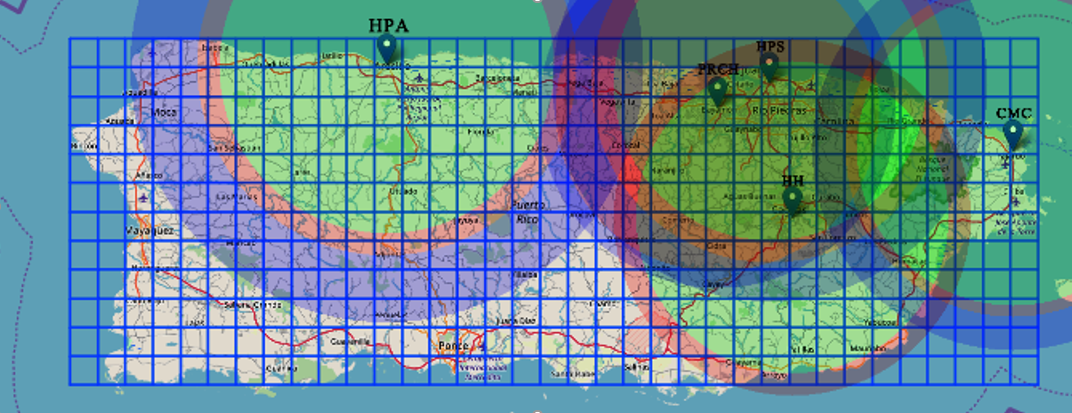
\includegraphics[width = 1\textwidth]{hcc.png}        
    	\caption{Concentric Circles Centered on Five Hospitals}                           
    	\label{hcc}                                          
    \end{figure}

	In Figure \ref{hcc}, blue circles belong to B drone, red circles belong to C drone and green circles belong to F drone. The circles for B drone centered in Hospital HIMA and for F drone centered in Puerto Rico Children's Hospital are lost because the drone can't fly too far or can't carry all the medical supply needed by the hospital in that situation.
	\par
	There is another dimension: on the basis of section \ref{ldis}, B Drone has the maximum performance. As a result, we will take B Drone into next localization calculation - cruising task is primarily responsible by B Drone. Now let's focus on the \textbf{flight paths}.
	\par
	\begin{description}
		\item[Path 1] Drones leave the container and return back after carrying out the reconnaissance mission. So the reconnaissance radius of each container is half of the maximum range of B drone. We can draw three circles with containers as the center and half of B drone's maximum range as the radius based on Figure \ref{thd2} (cover Puerto Rico and the high-weight grids as much as possible). Figure \ref{circle3} is our primary expectation.
		Here we have the inequality:
		\begin{equation}
		s=v*t_{max} \ge 2*s1 + s2   
		\end{equation}  
		Please note that here the drone is unloaded so the maximum journey distance s is represented by $v*t_{max}$ straight. 
		
		  \begin{figure}[H]                                         
			\centering
			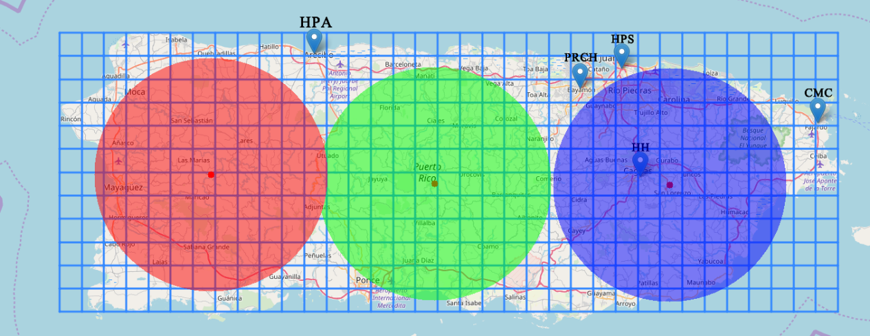
\includegraphics[width = 1\textwidth]{tcircle.png}        
			\caption{An Expected Localization Based on B Done}                           
			\label{circle3}                                          
		\end{figure}
		 \item[Path 2] Drones set out from a container and land in the contiguous container. In the figure above, if the two circles intersect or are tangent, some drones may have such flight trajectories, but this does not expand our scope of reconnaissance. Here we have the inequality:
		 		\begin{equation}
		 s=v*t_{max} \ge s1 + s2 + s3  
		 \end{equation}  
		 
		 \item[Path 3] Drones start out from a container and land in the hospital after finishing the reconnaissance missions (Assumption 6).  
		 \begin{Theorem} \label{thm:latex}
		 	The distance from any point P on the ellipse to the two focal points F1, F2, is equal to twice the length of the long axis $a$, namely $|PF_1|+|PF_2|=2a$.
		 \end{Theorem}
	 
	     According to the theorem above, for any point inside the ellipse, if we focus on the location of containers and hospitals, and take the maximum range of B drone as the long axis length - draw ellipses - then the region of all ellipses is the scope that drones can detect and eventually land in a hospital. Figure \ref{ellipses} shows the effect of one red ellipse for C drone, four green ellipses for F Drone and five blue ellipses for B Drone (use the same containers position as Figure \ref{circle3}). Figure \ref{circleE} shows the combination Figure \ref{circle3} and \ref{ellipses} which is our expected location map with the help of the grids weights concentration map (Figure \ref{thd2}). All the areas covered are reachable. 
	     
	        \begin{figure}[H]                                         
	     	\centering
	     	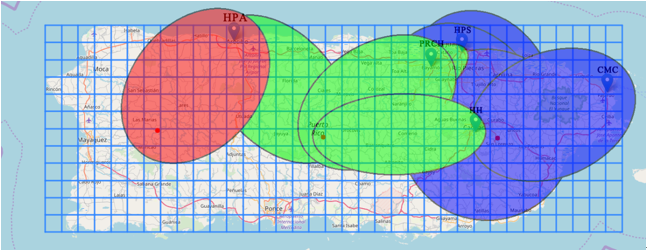
\includegraphics[width = 1\textwidth]{ellipses.png}        
	     	\caption{Useful Ellipses focused on Containers and Hospitals}                           
	     	\label{ellipses}                                          
	     \end{figure}
	     
	       \begin{figure}[H]                                         
	     	\centering
	     	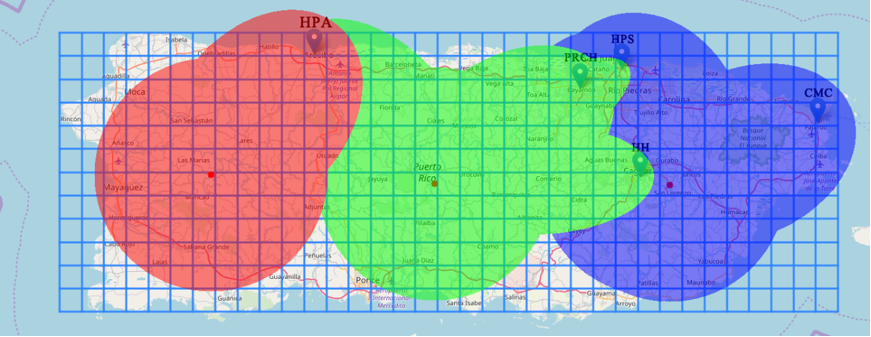
\includegraphics[width = 1\textwidth]{circleE.png}        
	     	\caption{Combination of Figure \ref{circle3} and \ref{ellipses} }                          
	     	\label{circleE}                                          
	     \end{figure}
	\end{description}

	In order to find the best location of three containers and evaluate our locations result, we set up two evaluation indicators: coverage ratio of grids number ($\alpha$), coverage ratio of grids weights ($\beta$). Their formula for calculation is as follows.
	\begin{align}
	\alpha&= \frac{C}{N} \\
	\beta&=\frac{{\sum\limits_{i = 1}^N {{G_i}{W_i}} }}{{\sum\limits_{i = 1}^N {{W_i}} }}
	\end{align} \par
   $G_i$ means the grid $i$, and $W_i$ means the weight or score of grid $i$. By traversing some probable locations and calculating $\alpha$ and $\beta$, we eventually locate three containers as the optimum localization: ( $(18.29^\circ, -66.97^\circ), (18.20^\circ, -66.50^\circ), (18.20^\circ, -65.97^\circ)$ ). There is about 0.005 degree deviation. Figure \ref{finallocation} shows the visual image. In this solution, the $\alpha=82.49\%$, the $\beta = 86.08\%$. Some blank areas are not covered because the weights of the grids are relatively small. More specifically, there maybe low population density, low traffic density or abominable geographical environment. \textcolor[rgb]{1.00,0.00,0.00}{Now, Problem \ref{P2} has been solved.}   
   
    \begin{figure}[H]                                         
   	\centering
   	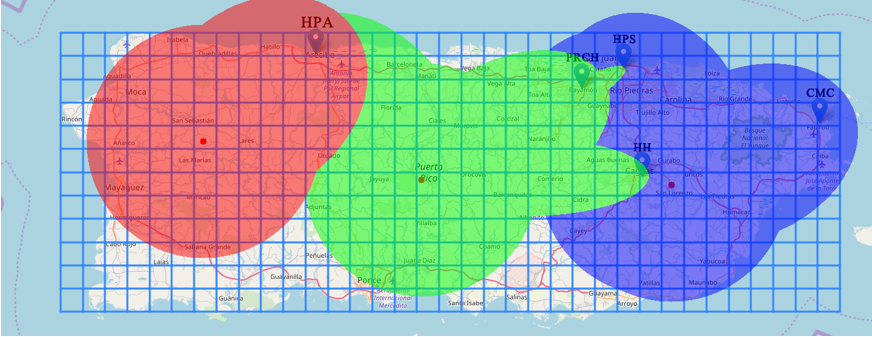
\includegraphics[width = 0.9\textwidth]{fcircleE.png}        
   	\caption{Final Optimum Localization}                          
   	\label{finallocation}                                          
   \end{figure}
     
      \section{Solution for Drone Flight Plan Based on Above Solutions  }

We stimulate the flight plan using \textbf{A*} Algorithm. Use the grids weights matrix as the Planning Environment Model of \textbf{A*}, and a grid can be a searching node of \textbf{A*}, since setting reasonable heuristic functions can benefit the selection of the node with minimum generation value as the node to be searched next. The essence of A* algorithm is the combination of greedy algorithm and heuristic search algorithm, so A* algorithm combines the advantages of both, and meanwhile inherits the characteristics of both. As a heuristic algorithm, A* algorithm has high search efficiency in path planning.  \par 
For A* algorithm, reasonable cost function design is the most important work. In the problem of route planning in drone defection, we consider that there are three quantities which have important influence on the final trace, then we design the cost function as follows: 
\begin{equation}
f(n)=g(n)+h(n)-m(n)
\end{equation}

 f (n) denotes the cost of the present node, g (n) denotes the distance traveled from the starting point to the present node, and m (n) denotes the total score obtained from the starting point to the present node. \par
 
  \begin{figure}[H]                                         
 	\centering
 	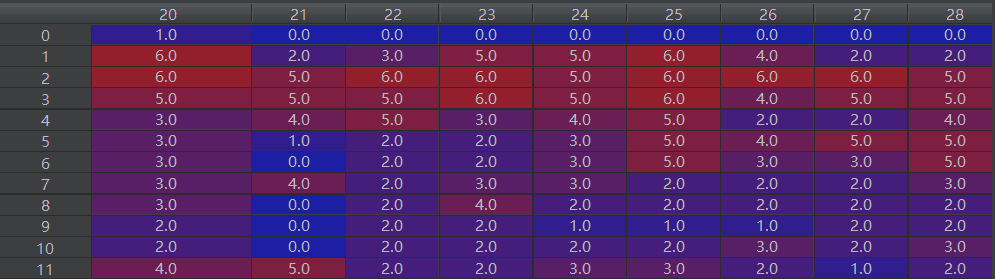
\includegraphics[width = 0.8\textwidth]{weightGrade.png}        
 	\caption{Grade Division Based Grids Weights Matrix (Figure \ref{finalweights})}                          
 	\label{gdbo}                                          
 \end{figure}
We normalize the weights in the grid weight matrix above and get a fractional matrix W in the fractional interval mapped to [0,6] (Figure \ref{gdbo}). Drones needs to move 5 km to fly over a grid horizontally or vertically, and 7 km to fly obliquely over a grid. Whatever way it flies over a grid, the score of the grid is equal to its original score minus three (the score is at least 0, it will not become negative). On this basis, we give: 
\begin{align}
g(j) &= g(i) + \sqrt {{{({x_i} - {x_j})}^2} + {{({y_i} - {y_j})}^2}} \\
h(j) &= \sqrt {{{({x_E} - {x_j})}^2} + {{({y_E} - {y_j})}^2}} \\
m(j) &= m(i) + \left\{ \begin{array}{l}
3,if{w_j} \ge 3\\
{w_j},if{w_j} < 3 
\end{array} \right\}
\end{align}
 I is the current node and j is a neighbor node of I. E is the midpoint and W is the fraction. \par
 The implementation process and summary of A* algorithm in path planning are as follows: starting from the starting point, searching the point with the lowest cost function value in the neighborhood node, expanding gradually outward until the end of the algorithm search. Firstly, starting from the starting point and the starting point is stored in the open set and all the nodes in its neighborhood are scanned to calculate the $f(j)$ value of their grid nodes in all the neighborhood nodes and coexist. The $f(j)$ calculated are stored in the open set. After completing the node expansion of the starting point, we delete the starting point from the open set and join it into the closed set. Select the candidate node with the lowest $f(j)$ value in the open set as the temporary path point, and point the pointer of the current node to the new node, then we complete the establishment of the second temporary path point. After that, we start the new node expansion. The next is the process for realization \cite{7}.
 
     	    \begin{algorithm}
 	\label{al4}
 	\renewcommand{\algorithmicrequire}{\textbf{Input:}}
 	\renewcommand{\algorithmicensure}{\textbf{Output: }}
 	\caption{Pseudo Code for Flight Plan}
 	\begin{algorithmic}[2]
 		\REQUIRE  The weight matrix $W$.
 		\ENSURE The path set of drone start from three containers. 
 		\STATE  Step1: Denote the P container as the starting point. 
 		\STATE Step2: Select a point within the container coverage as the end point of the A* algorithm. 
 		\STATE Step3: Run A* algorithm to get the best path and record the score mE of the path 
 		\STATE Step4: Repeat Step3 and Step4 to find the path with the highest score, record the path, and modify the score of the node through which the path passes. 
 		\STATE Step5: Repeat Step5 until you find all the paths starting from this container. 
 		\STATE Step6: Repeat Step2 to get the path set of three containers. 
 		\STATE \textbf{return} the Path Set.
 	\end{algorithmic}  
 \end{algorithm}
The result of running this algorithm is: $\alpha$=71.27\%, $\beta$= 83.61\%.

Taking terrain factors into account, we mark some unreachable areas with yellow and set their grades to zero. Then we get Figure \ref{gcla}.
 \begin{figure}[H]                                         
 	\centering
 	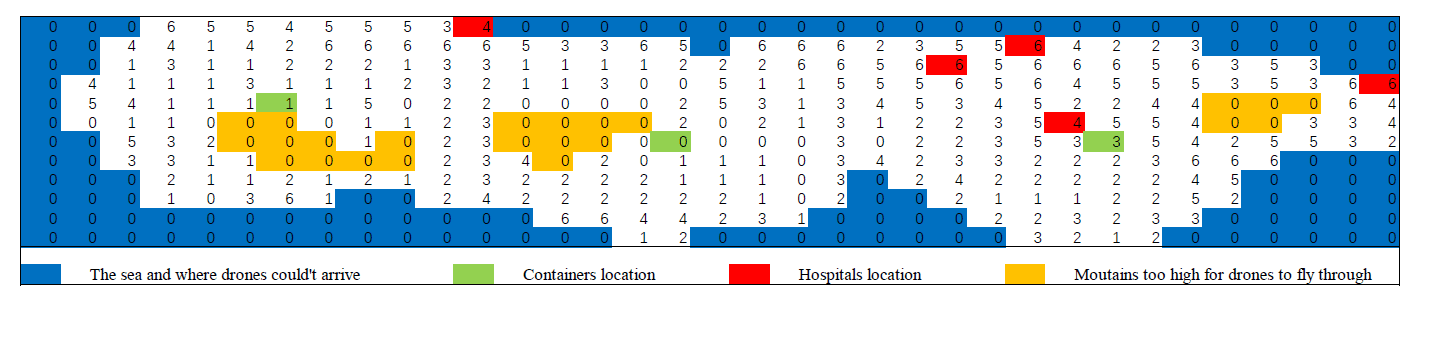
\includegraphics[width = 0.9\textwidth]{detailGrids.png}        
 	\caption{Grids Classification}                          
 	\label{gcla}                                          
 \end{figure}
We give priority to high-ranking grids and do resource allocation mainly on grids with grade 5 and 6, only to find no more than 20 B drones are needed for each containers. Figure \ref{pfp} shows the detail. 
\begin{figure}[H]                                         
	\centering
	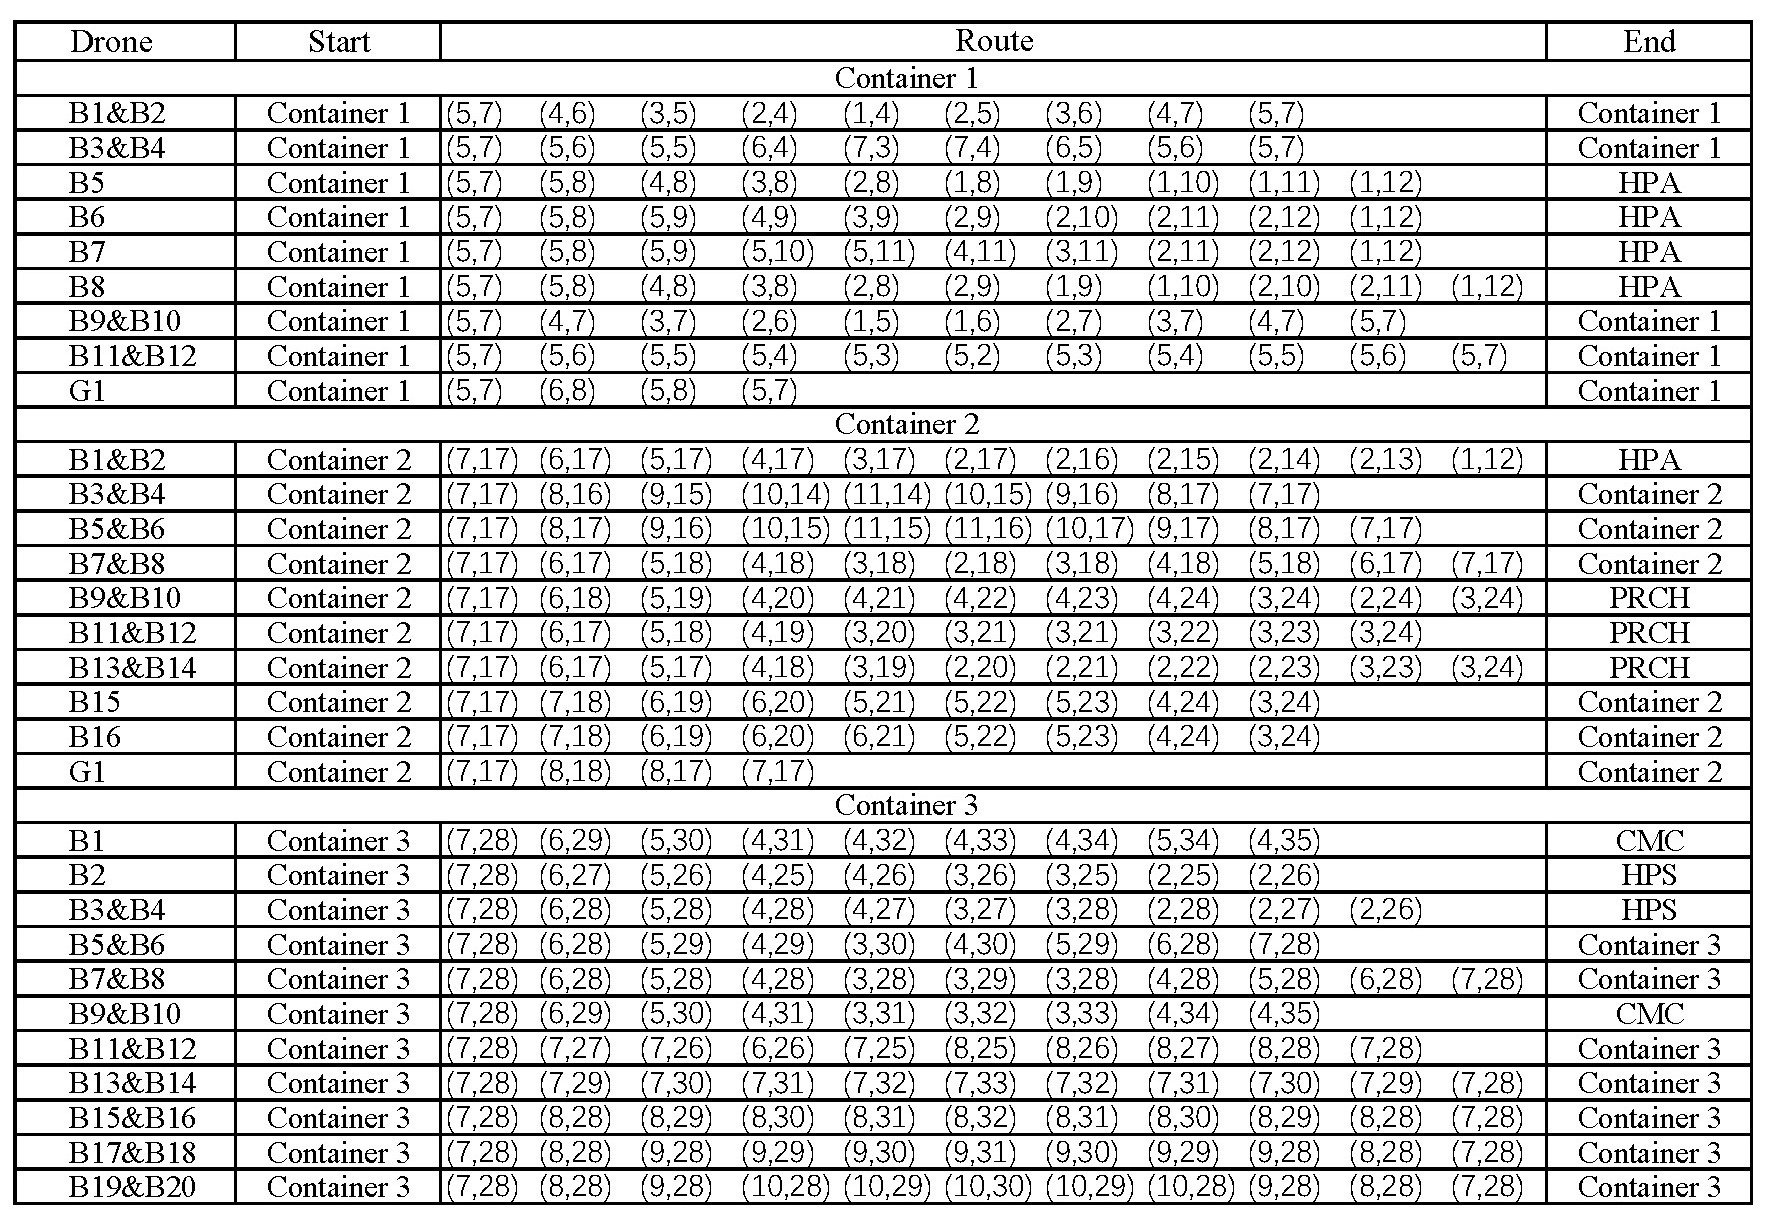
\includegraphics[width = 1\textwidth]{plan.jpg}        
	\caption{A Part of Fight Plan Covering Grids of Grade 5 and 6}                          
	\label{pfp}                                          
\end{figure}
    
    The next figure are concrete flight routes starting from three containers. The thicker the line is, the drone fleet bigger. \textcolor[rgb]{1.00,0.00,0.00}{Now, Problem \ref{P4} has been solved.}   
    \begin{figure}[H]                                         
    	\centering
    	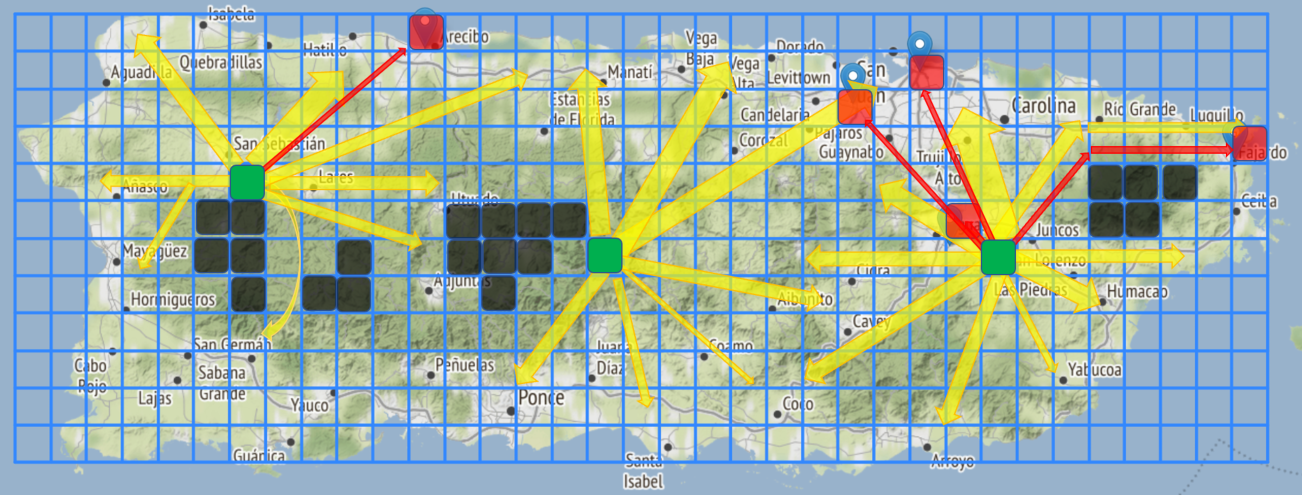
\includegraphics[width = 1\textwidth]{routes.png}        
    	\caption{A Sketch Map Showing Drone Routes}                          
    	\label{pfpss}                                          
    \end{figure}
    
%            \begin{table}[H]
%        	\centering
%        	\caption{The Different Layer of The Forty Countries}
%        	\label{ceng}
%        	\begin{tabular}{cccccccll}
%        		\toprule
%        		Hierarchy                & \multicolumn{5}{c}{Country}                                   \\
%        		\midrule
%        		The First Network Layer  & America      & Mexico      & Russian     & Ukraine  & India     \\
%        		& Germany      & China       &             &          &          \\
%        		\midrule
%        		The Second Network Layer & Bangladesh   & Pakistan    & U.K         & France   & Canada    \\
%        		& Italy        & Philippines & Iran        &          &           \\
%        		\midrule
%        		The Third Network Layer  & Turkey       & Spain       & Afghanistan & Algeria  & Poland   \\
%        		& Morocco      & Japan       & Viet Nam    & Korea    &           \\
%        		\midrule
%        		The Forth Network Layer  & Brazil       & Colombia    & Argentina   & Iraq     & Congo   \\
%        		& South Africa & Nigeria     & Thailand    & Tanzania & Myanmar   \\
%        		& Indonesia    & Sudan       & Egypt       & Kenya    & Uganda   \\
%        		& Ethiopia     &             &             &          &          \\
%        		\bottomrule
%        	\end{tabular}
%        \end{table}
%    
%        \begin{table}[H]
%        	\centering
%        	\caption{The Predictions of 6th-16th Language`s Total Numbers of Speakers}
%        	\label{Bdaan}
%        	\begin{tabular}{ccccccc}
%        		\toprule
%        		& \multicolumn{2}{c}{L1} & \multicolumn{2}{c}{L2} & \multicolumn{2}{c}{Total} \\
%        		\midrule
%        		& Now    & In 50 Years   & Now    & In 50 Years   & Now     & In 50 Years     \\
%        		Malay      & 77     & 107           & 204    & 271           & 281     & 378             \\
%        		Bengali    & 242    & 340           & 19     & 22            & 261     & 362             \\
%        		Russian    & 153    & 183           & 113    & 158           & 267     & 341             \\
%        		Portuguese & 218    & 297           & 11     & 16            & 229     & 313             \\
%        		French     & 76     & 101           & 153    & 203           & 229     & 304             \\
%        		Hausa      & 85     & 132           & 65     & 93            & 150     & 225             \\
%        		Punjabi    & 148    & 192           &        &               & 148     & 192             \\
%        		German     & 76     & 106           & 52     & 69            & 129     & 175             \\
%        		Persian    & 60     & 84            & 61     & 85            & 121     & 169             \\
%        		Japanese   & 128    & 164           & 1      & 1.3           & 129     & 165.3           \\
%        		Swahili    & 16     & 22            & 91     & 131           & 107     & 153\\
%        		\bottomrule
%        	\end{tabular}
%        \end{table}
    
    
    \section{Model Rationality  Analysis}
    
    \begin{itemize}
    	\item Grids number coverage rate $\alpha$ is smaller than grids weight coverage rate, which validate our grids weights matrix in \textbf{GTM} (section \ref{finalweights}).
    	\item Each grid is a square 5 km on a side while the breadth of vision of drones is about 2770 m. A drone only needs to have a 10 km flight for reconnoitring a whole grid.
    	\item The results indicate our whole packing configuration can achieve the entire reconnaissance task of the marked area in Figure \ref{finallocation}, which means our models and solutions are reliable.
    	\item \textbf{Sensitivity Analysis}: We reconsider the factors affecting the grids - calculate grids weights with only one factor independently - and finally obtain the following comparison map.
    	    \begin{figure}[H]                                         
    		\centering
    		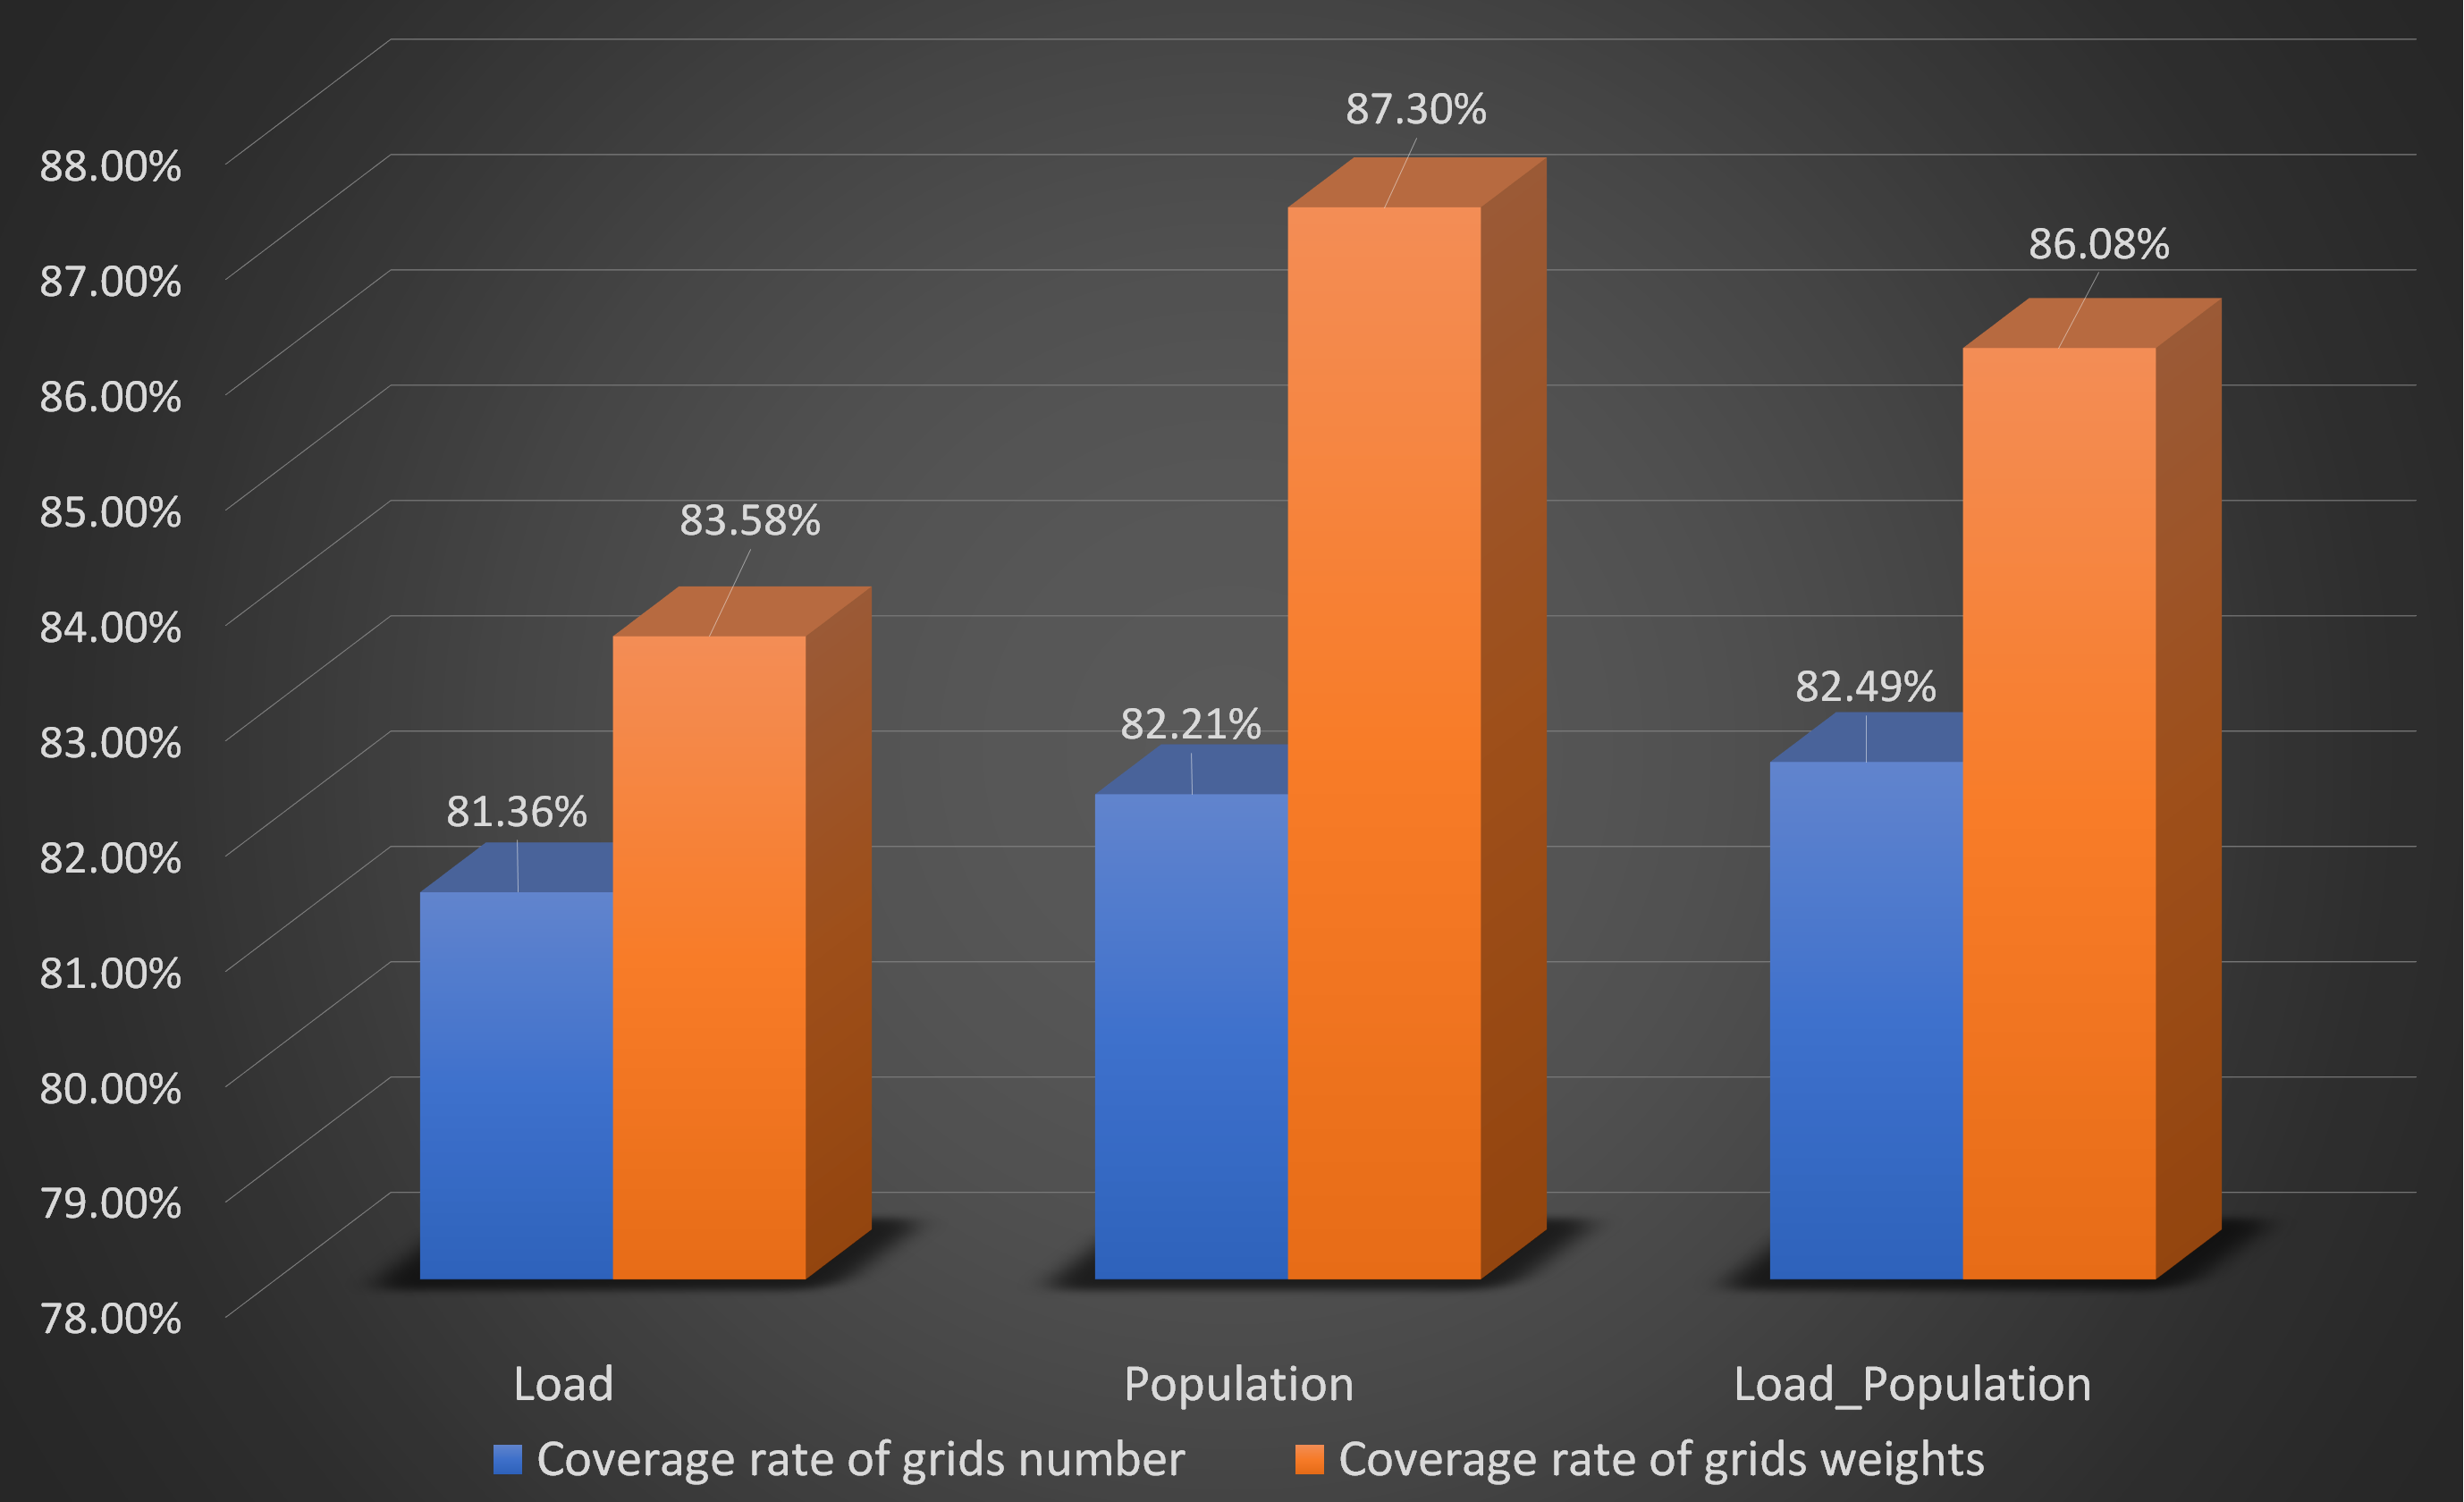
\includegraphics[width = 0.8\textwidth]{exam.png}        
    		\caption{Sensitivity Analysis on Different Affecting Factor of Grids Weights}                          
    		\label{pf}                                          
    	\end{figure}
    \end{itemize}
    
%    \subsection{Error Analysis}
%     \begin{itemize}
%    	\item
%    	\item
%    	\item
%    \end{itemize}
    
    
    \section{Strengths and Weaknesses}
    \subsection{Strengths}
    \begin{itemize}
    	\item The grids traversing model (GTM) is a basis of all the models, which achieves the quantization of real problems properly. 
    	\item GTM adopts traffic highway density, population density and topographic factor to evaluate the weights of grids reasonably.
    	\item The entropy weighting model (EWM) makes full use of information entropy to weigh different indexes scientifically, which is propitious to identify pivotal grids and screen out meaningless area. 
    	\item The optimum localization model (OLM) centers on hospital and draw ellipses and circles, considering most of the probabilities and converting their into math model.
    \end{itemize}
    \subsection{Weaknesses}
    \begin{itemize}
    	\item Enormous uncertain variables entail our models hard to be examined.
    	\item It's difficult to realize GTM and solve the flight plan perfectly under such limited time. 
    	\item The final solution of packing configuration, and localization is given too roughly and lacking validation, while the detailed process is too tedious to say. 
    \end{itemize}

\begin{thebibliography}{99}                
	\bibitem{1} Zhenji Ding. Research on Emergency Relief Task Assignment Technology of Multi-UAV in Urban Environment [D].Nanjing: Nanjing University of Aeronautics and Astronautics, 2016. 
	\bibitem{2} Yaqian Zhang. Study on Road Network Density Based on Land Volume Ratio[D]. JiNan: Shandong Jianzhu University, 2018.
	\bibitem{3} \href{https://en.wikipedia.org/wiki/Municipalities_of_Puerto_Rico#cite_note-census-2010-11?tdsourcetag=s_pcqq_aiomsg} {Population Data of Puerto Rico's City} (This is a hyperlink and you can click it directly.)
	\bibitem{4} \href{https://en.wikipedia.org/wiki/Puerto_Rico#Population_makeup}{Puerto Rico's Total Population Data Over the Years}
	\bibitem{5} Guanhong Wu, Jiaming Zhu. Evaluation of Urban Livability in Huaihai Economic Zone Based on Entropy Weight Method [J].Journal of Hunan City College, 2018, 27(3): 42-45. 
	\bibitem{6} Haoyuan Hu, Xiaodong Zhang. Solving a New 3D Bin Packing Problem with Deep Reinforcement Learning Method. Hangzhou, 2017.
	\bibitem{7} Zhonghua Han, Xinghao Feng, Lu Zhe, Yang liying, An Improved UAV Path Planning Environment Modeling Method[j], Information and Control,2018,47(03):371-378.
\end{thebibliography}

\section{Memo}

\noindent TO: Dear Madam  \\
From: A Modeling Team  \\
Subject: Results, Conclusions and Recommendations about 'DroneGo'  \\

Dear madam, we are honored to contribute to the disaster relief work you have done. Here are our results, conclusions and recommendations about 'DroneGo' system designed by our model.

\textbf{Results}
To develop a DroneGo disaster response system to support the Puerto Rico hurricane disaster scenario, we need three ISO cargo con trainers to cover most of the islands (area coverage: 82.49\% and weighted area coverage: 86.08\%). And one at(18.29$\pm$ 0.005$^\circ$N; 66.97$\pm$0.005$^\circ$W), one at(18.20$\pm$0.005$^\circ$N; 66.50$\pm$0.005$^\circ$W), and the last at (18.20$\pm$0.005$^\circ$N;\\ 65.97$\pm$0.005$^\circ$W).
As for medical packages allocation, we first ensure that we can supply the three-day supply of the five hospitals on the island and assign tasks to the corresponding containers according to the positioning of the containers. Based on the drone evaluation, we have determined the most suitable type of drone for packages delivery and reconnaissance. Combined with the above modeling results, the container task and the drone transport fleet are configured as follows:
	\begin{table}[H]
	\centering
	
	\begin{tabular}{lllcc}
		\cline{1-5}
		
		\multicolumn{1}{c}{Hospital (abbr.)}  & \multicolumn{1}{c}{Container}         & \multicolumn{1}{c}{Drone} & \multicolumn{1}{c}{Distance (km)}     & \multicolumn{1}{c}{Fight Time (hour)} \\
		\cline{1-5}
		
		\multicolumn{1}{c}{CMC}  & \multicolumn{1}{c}{3}  &\multicolumn{1}{c}{B: 1$\times$3}    & 36 & 0.55   \\
		\multicolumn{1}{c}{HH}   & \multicolumn{1}{c}{3}  &\multicolumn{1}{c}{E: 1$\times$3}    & 7 &  0.14  \\
		\multicolumn{1}{c}{HPS}  & \multicolumn{1}{c}{3}  &\multicolumn{1}{c}{B: 1$\times$3}  & 27 & 0.39 \\ 
		\multicolumn{1}{c}{PRCH} & \multicolumn{1}{c}{3}  &\multicolumn{1}{c}{B: 1$\times$3;  C: 1$\times$3}  & 28 & B: 0.448; C: 0.494     \\
		\multicolumn{1}{c}{HPA}  & \multicolumn{1}{c}{1}  &\multicolumn{1}{c}{B: 1*3}   & 32  & 0.43  \\ 			
		\cline{1-5}
		
	\end{tabular}
	\caption{Drone Payload Packing Configuration and Schedule}

\end{table}

When resolving reconnaissance missions, we use the B-type drone with the highest reconnaissance evaluation score to perform the reconnaissance mission according to the modeling results. Then we found that the number of unmanned aerial vehicles that can be loaded in the remaining space of the container far exceeds the model planning needs, resulting in wasted container space. See the table below for details: 

\begin{table}[H]
	\centering
	
	\begin{tabular}{llll}
		\cline{1-4}
		
		\multicolumn{1}{c}{Container}  & \multicolumn{1}{c}{Position} & \multicolumn{1}{c}{Drone Configuration} & \multicolumn{1}{c}{Medical Kits Configuration} \\ 
		\cline{1-4}
		
		\multicolumn{1}{c}{1} & \multicolumn{1}{c}{$(18.29^\circ N, 66.97^\circ W)$} & \multicolumn{1}{c}{B:75 G:1 H:1}    &  $M_1\times3+M_n\times n$     \\
		\multicolumn{1}{c}{2} & \multicolumn{1}{c}{$(18.20^\circ N, 66.50^\circ W)$} & \multicolumn{1}{c}{B:75 G:1 H:1}   &   $M_n \times n$      \\
		\multicolumn{1}{c}{3} & \multicolumn{1}{c}{$(18.20^\circ N, 65.97^\circ W)$}  &\multicolumn{1}{c}{B:61 C:3 E:3 H:1}   &  $M_1\times 18+M_2\times 6 +M_3 \times 12 +M_n\times n$ \\ 
		
		\cline{1-4}
		
	\end{tabular}
	\caption{Packing Configuration for Three Containers}

\end{table}

\textbf{Conclusions}
The system designed by our model can finish the medical supply delivery task in 0.55 hours (33 mins), which will ensure that people in the disaster area can get help in the first time when your organization arrives.
In the video reconnaissance task, it is sad that this system could not cover the whole main island of Puerto Rico. In our model, we not only consider the factors of the roads, but also the factors of the population, which make our designed system has a better performance than only considering factor of roads.

\textbf{Recommendations } \\
In order to cover more area, some schemes are proposed: 

1.	Prepare more containers. In the Puerto Rico hurricane scenario, we believe that more than 95\% area could be covered with one more container.
 
2.	Prepare better drone. According to the information we have consulted, there are drones that could fly longer distance than the drones provided in this problem. With a larger max voyage, every container could handle a large area.

3.	Set more drone landing points. The problem that there are no more options for landing points has always perplexed us. Drones will not have to fly back to the containers any more with more landing points, which will double the voyage of the drones.

4.	The drone fleet and medical packages contained in each container has exceeded demand. Smaller containers will be more suitable.
 
5.	If this system is going to be used in other scenarios, local topography is an important factor to be considered to decide the locations.

\newpage
    \begin{appendices}
    	\section{Algorithms 3 and 4}
%    	\subsection{Least Surface Area Heuristic}
    	    \begin{algorithm}
    		\label{al2}
    		\renewcommand{\algorithmicrequire}{\textbf{Input:}}
    		\renewcommand{\algorithmicensure}{\textbf{Output: }}
    		\caption{Least Surface Area Heuristic}
    		\begin{algorithmic}[2]
    			\REQUIRE  The set of collection of residues ($I$), volume of cargo ($V$).
    			\ENSURE The item i to be loaded.
    			\STATE  Denote the set of empty maximal space as $ES$, the set of orientations as $O$. 
    			\STATE Initialize the least surface area for item i as $LSA_i=3*(max(l_i,w_i,h_i)*n)^2$.
    			\STATE Initialize best empty maximal space $s'_i=null$, best orientation as $o'_i = null$. 
    			\FORALL {each empty maximal space $S \in ES$ }
    			\FORALL {each orientation $o\in O$}
    			\STATE Calculate the surface area  $SA_{}i,s,o$  after putting item i in empty maximal space s with orientation o. 
    			\STATE   \textbf{if} $SA_{i,s,o} < LSA_i$ \textbf{then}
    			\STATE   Update $s'=s, o'=o$ and $LSA_i\leftarrow SA_{i,s,o}$.
    			\STATE \textbf{else if} $SA_{i,s,o}+LSA_i$ \textbf{then}
    			\STATE  Apply the tie-breaking rule. (Selecting s,o if and only if min(length(s)-o($l_i$), width(s)-o($W_i$), height(s)-o($h_i$)) is less than min(length($s_i$)-$o_i(l_i)$, width($s_i$)- $o_i(w_i)$, height($s_i$)-$o_i(h_i))$, where length(s), width(s), height(s) represents the length, width, height of empty maximal space s and o($l_i$), o($w_i$), o($h_i$) represents the length, width, height of item i with orientation o.) 
    			
    			\STATE \textbf{end if}
    			\ENDFOR
    			\ENDFOR
    			\STATE \textbf{return} $s'_i, o'_i$ for item i.
    		\end{algorithmic}  
    	\end{algorithm}
    	
%    	\subsection{Least Waste Space Heuristic}
    	\begin{algorithm}
    		\label{al3}
    		\renewcommand{\algorithmicrequire}{\textbf{Input:}}
    		\renewcommand{\algorithmicensure}{\textbf{Output: }}
    		\caption{Least Waste Space Heuristic}
    		\begin{algorithmic}[1]
    			\REQUIRE Remaining items as I', volume of item i as $V_i$.
    			\ENSURE Location and orientation of items in space.
    			\STATE  Initialize the best item $i' =null$.
    			\STATE  Initialize the least volume as $LV = {(max({l_i},{w_i},{h_i}){\rm{\cdot}}n)^3}$
    			\FORALL {each item $i\in I'$ }
    			\STATE   Calculate the volume V after packing item i according to $s'_i, o'_i$ (which is determined by Least Surface Area Heuristic). Denote the least waste space of item $LWV_i = V-V_i$. 
    			\STATE   \textbf{if} $LWV_i<LV$ \textbf{then}
    			\STATE Update $LV=LWV_i$.
    			\STATE Update $i'=i$.
    			\STATE \textbf{end if}
    			
    			\ENDFOR
    			
    			\STATE \textbf{return} $s'_i, o'_i$.
    		\end{algorithmic}  
    	\end{algorithm}
    
    	\section{Codes in Python}
    	
    	The following codes are \textbf{parts} of related programs written in Python.  \par
    \textbf{Draw Map of Puerto Rico with Grids: }
    \lstinputlisting[language=Python,breaklines]{./code/feature.py} \par
      \textbf{3D Packing Optimization Problem:} (Cite and modify from resource on Github ) 
    \lstinputlisting[language=Python,breaklines]{./code/main_copy.py}
     \textbf{Calculating Weights of Grids and Drones:} 
    \lstinputlisting[language=Python,breaklines]{./code/weight.py}
    \lstinputlisting[language=Python,breaklines]{./code/UAV_weight.py}
    \section{Codes in Matlab}
    The following codes are \textbf{parts} of related programs written in Matlab.  \\
    
%    	\textbf{\textcolor[rgb]{0.98,0.00,0.00}{Input matlab source:}}
%    \lstinputlisting[language=Matlab]{./code/mcmthesis-matlab1.m}
     \textbf{Draw pictures:} 
     \lstinputlisting[language=Matlab,breaklines]{./code/TransferAFiletoThreeColumns.m}
    \lstinputlisting[language=Matlab,breaklines]{./code/humanDensity.m}
    \lstinputlisting[language=Matlab,breaklines]{./code/TrafficDensityMap.m}
    \lstinputlisting[language=Matlab,breaklines]{./code/weight_map.m}
    
    \section{Codes in C++}
    The following codes are related programs written in C++. \par
    \textbf{Generate parameters for python drawing:} 
    \lstinputlisting[language=C++,breaklines]{./code/stringForPython.cpp}
    	
    \end{appendices}

\end{document}


\end{document}
